\documentclass[12pt, letterpaper]{report}

%%%%%%%%%%%%%%%%%%
% -- Packages -- %
%%%%%%%%%%%%%%%%%%

% UTF8 encoding
\usepackage[utf8]{inputenc}

% Graphics and path to graphics
\usepackage{graphicx}
\graphicspath{ {figures/} }

% Colors, especially for highlighting and editing
\usepackage[usenames, dvipsnames]{color}

% Margins, links etc..
\usepackage[letterpaper, margin=1in]{geometry}
\usepackage{hyperref}
\hypersetup{
  colorlinks   = true,  %Colours links instead of ugly boxes
  urlcolor     = blue,  %Colour for external hyperlinks
  linkcolor    = black, %Colour of internal links
  citecolor    = black   %Colour of citations
}
\usepackage{setspace}

% Math packages
\usepackage{amsmath}
\usepackage{array}
\usepackage{mathtools}
\usepackage{enumitem}

% Page alignment \addtolength{\hoffset}{0pt}
\addtolength{\voffset}{0pt}

%%%%%%%%%%%%%%%%%%%%%%%%%%%%%%
% -- Aliases and commands -- %
%%%%%%%%%%%%%%%%%%%%%%%%%%%%%%

\renewcommand{\d}{\delta}       % Dirac delta
\newcommand{\F}{\mathcal{F}}    % Free energy Functional
\renewcommand{\l}{\left}        % Quick left
\renewcommand{\r}{\right}       % Quick right
\newcommand{\f}{\frac}          % Quick fraction
\newcommand{\Z}{\mathcal{Z}}    % GC partition function
\newcommand{\D}{\mathcal{D}}    % Swirly D for path integrals
\newcommand{\fphi}{\tilde{\phi}}% Fourier space phi
\newcommand{\fh}{\tilde{h}}     % Fourier space h
\newcommand{\fxi}{\tilde{\xi}}  % Fourier space xi
\newcommand{\A}{\rho_A}         % Density of species A
\newcommand{\B}{\rho_B}         % Density of species B
\newcommand{\ham}{\mathcal{H}}  % Hamiltonian (classical)
\newcommand{\q}{\mathbf{q}}     % Phase space coordinates
\newcommand{\p}{\mathbf{p}}     % Phase space momenta

% Plane wave + and -
\newcommand{\pwp}{e^{\frac{i\mathbf{p}\cdot\mathbf{q}}{\hbar}}}
\newcommand{\pwm}{e^{-\frac{i\mathbf{p}\cdot\mathbf{q}}{\hbar}}}

% Classical Trace
\newcommand{\trace}[1]{\mathrm{Tr}\left[ #1 \right]}

% Average
\newcommand{\mean}[1]{\left\langle #1 \right\rangle}

% Integral
\newcommand{\integrate}[1]{\int \mathrm{d}#1\,}

%%%%%%%%%%%%%%%%%%
% Document Begin %
%%%%%%%%%%%%%%%%%%

\pagenumbering{roman}

\begin{document}

%%%%%%%%%%%%%%%%%
%  Front Matter %
%%%%%%%%%%%%%%%%%

\begin{titlepage}
    \begin{center}
        \vspace*{1cm}
        
        \Huge
        \textbf{
            Thesis Title
        }
        
        \vspace{0.5cm}
        \LARGE
        Thesis Subtitle
        
        \vspace{1.5cm}
        \Large 
        \textbf{Nathan Frederick Smith}
        
        \vfill

        \Large
        A thesis presented in partial fulfillment of the degree of\\
        Master's of Science
        
        \vspace{0.8cm}
        
        
\includegraphics[width=0.2\textwidth]{crest.eps}
        
        \Large
        Department of Physics\\
        McGill University, Montreal\\
        Canada\\
        ??-??-2017
        
    \end{center}
\end{titlepage}

\doublespacing

\section*{Dedication}
\label{sec:dedication}
\addcontentsline{toc}{chapter}{\nameref{sec:dedication}}

Dedication here...

\clearpage

\section*{Acknowledgements}
\label{sec:acknowledgements}
\addcontentsline{toc}{chapter}{\nameref{sec:acknowledgements}}

Acknowledgements here...

\clearpage

\section*{Abstract}
\label{sec:abstract}
\addcontentsline{toc}{chapter}{\nameref{sec:abstract}}

English abstract...

\clearpage

\section*{Abrégé}
\label{sec:abrege}
\addcontentsline{toc}{chapter}{\nameref{sec:abrege}}

French abstract...

\clearpage

\tableofcontents 
\listoffigures
\listoftables

%%%%%%%%%%%%%%%%%%%%%
% -- Main Matter -- %
%%%%%%%%%%%%%%%%%%%%%

\chapter{Introduction}
\label{introduction}
\pagenumbering{arabic}
\label{chapter:introduction}

% Thesis introduction outline: https://student.unsw.edu.au/introductions

% 1) State the general topic and give some background

The study of two binary alloys in materials physics is a pursuit of incredibly
broad impact. Industries as distant as the large commerial materials such as
steel and aluminium producers and burgeoning markets of nano-fabrication and
optoelectronics are affected by research in binary alloys.

One suprising aspect of binary alloys is the rich diversity of properties and
behaviours they display. Because material properties depend on the
microstructural details of the material they have a strong path dependence.
Grain boundaries, vacancies, dislocations and other microstructural are all
intimitly tied to the manufactoring process of the alloy. This means that the
study of solids can never be completely seperated from the study of
solidification. As such the diversity of material properties and behaviours we
see in binay alloys can be directly attributed to the diversity of processes
for their construction.

Given the importance of these systems it is important to construct models that
can explain diversity of behavior we see in them. At the moment models of
solidification can be categorized by the length and time scales they accurately
discribe. The the macroscopic length and time scales we have continuum methods
of heat and mass transport and associated finite element methods of analysis.
These methods are appropriate for studying large castings for example. On
length scales $\mathcal{O}(10^{-3})m$ to $\mathcal{O}(10^{-6})$ we use
\textit{Phase Field} methods to study phenomena such as dendritic growth and
chemical segregation. On still finer length scales from $\mathcal{O}(10^{-9})$
to $\mathcal{O}(10^{-6})$ and on relatively long timescales we have the methods
of \textit{Phase Field Crystal} theory and dislocation dynamics. These methods
are appropriate for studying nanoscopic changes that occur on diffusive
timescales such as dislocation motion, creep, grain boundary motion and micro
segregation. At a still finer scale and on very short time scales
($\mathcal{O}(10^{-12}s)$) we have the methods of molecular dynamics and
density functional theory. This methods are appropriate for the study of
transport coefficients and interaction potentials.

% 2) Outline the current situation

In this thesis we'll focus on the binary Phase Field Crystal (PFC) theory. The 
binary phase field crystal theory has been successful in describing a broad
selection of phenomena in binary alloys. These successes include the Kirkendall
effect \cite{ELDER11_KIRKENDALL, LU15}, solute drag \cite{GREENWOOD12}, 
clustering and precipitation \cite{FALLAH12, FALLAH13, FALLAH13_AlCu_experiment},
colloidal ordering in drying suspensions \cite{GANAI13}, epitaxial growth
and island formation \cite{ELDER10_NANOISLAND, LU16}, and ordered crystals
\cite{ALSTER17} to name a few. 

The PFC theory is derived from Classical Density Functional Theory (CDFT) and as
such it is a sort of simplified density functional theory. In practice,
two different variants of the PFC theory are used in practice: The original
model developed by Elder \textit{et al} \cite{ELDER07} and the Structural
Phase Field Crystal (XPFC) model developed by Greenwood \textit{et al.}
\cite{GREENWOOD11_BINARY}. The original model is a very reduced form of
CDFT and so it lacks completeness in its ability to describe binary alloys.
Specifically, the original model uses an expansion in concentration that limits 
its ability to describe a realistic phase diagram. The original model also
uses a very simplified correlation kernel which limits its ability to describe
a variety of crystal lattice structures. The XPFC model is an improvement 
in that is ameliorates both of these problems. The concentration is left 
unexpanded allowing for construction of realistic global phase diagrams instead
of local expansions. The XPFC model provided a phenomenology for modelling
correlation functions that succeeded in describing solidification of a
variety of lattice structures ({\color{ForestGreen} Find that paper about
solidification of all 2d lattices}). 

% 3) Evaluate the current situation and identify a gap

In introducing its phenomenology for modelling correlation function, the 
XFPC theory tacitly assumes that there is some preferred structure at high
concentration and some other structure preferred at low concentration. This
can be limited in situation that have a specific structure specifically at intermediate
concentrations such a syntectic material. The XPFC model also assumes no
long wavelength correlations in the concentration field which in practice means
the model has an ideal free energy of mixing. This is another limitation of 
the XPFC model because in general the enthalpy of mixing is not zero for 
binary alloys.

% 5) State the research goals and aims

This goal of the current research is to present two improvements to the
binary XPFC theory. The first improvement is a more general phenomenology
for modelling pair correlation functions of a material. The second 
improvement is two extend the free energy of mixing beyond ideality to 
account for circumstances when the heat of mixing is not negligible.

% 6) Outline the order of information

This thesis is divided into 6 chapters:
%
\begin{description}
    \item [Chapter \ref{chapter:cdft_intro}] { Classical Density Functional
        Theory (CDFT) is introduced and derived from fundamental principles of
        quantum statistical mechanics.
    }
    \item [Chapter \ref{chapter:cdft_of_freezing}] { CDFT theory of
        solidification is described and discussed. The density functional
        theory is extended to a dynamic, non-equilibrium theory and the Phase
        Field Crystal (PFC) Theory is introduced as a simplified density
        functional theory.
    }
    \item [Chapter \ref{chapter:binary}] { Binary PFC theory is established and
        previous simplified models are summarized and discussed.
    }
    \item [Chapter \ref{chapter:improvements}] { Improvements to the XPFC model
        are discussed and contains novel contribution to the field.
    }
    \item [Chapter \ref{chapter:applications}] { Concludes the thesis by
        applying the improved XPFC model to the problem of multistep nucleation
        of nanoparticles and discusses potential future applications.
    } 
\end{description}
%



\chapter{Introduction to Classical Density Functional Theory}
\label{chapter:cdft_intro}

Many physical theories are derived using a succession of approximations. While
each approximation yields a theory that is more narrow in scope, it is
typically more tractable to either analytical or numerical analysis.  Classical
Density Functional Theory (CDFT) is derived using this approach and in this
chapter we'll examine each approximation and the intermediate theory they
supply. 

CDFT is a theory of statistical mechanics. This means CDFT connects microscopic
physics to macroscopic observables using statistical
inference\footnote{Statistical mechanics is not always described as statistical
inference. See works of E. T. Jaynes for details on this approach
\cite{JAYNES57}} instead of attempting to compute microscopic equations of
motion. The microscopic physics in this case is most accurately described by
many-body quantum mechanics and so the theory of quantum statistical mechanics
is a natural starting point in any attempt to calculate thermodynamic
observables.

We will see that for our systems of interest that the full quantum statistical
theory is completely intractable. To preceed, we'll look at quantum statistical
mechanics in the \textit{semi-classical limit}. In the semi-classical limit
we'll develop a theory of inhomogenous fluids called Classical Density
Functional Theory (CDFT). Finally, we'll see that constructing exact free
energy functionals for CDFT is rarely possible and look at an approximation
scheme for these functionals.

%%%%%%%%%%%%%%%%%%%%%%%%%%%%%%%%%%%%%%%%%%%%%%%%%%%%%%%%%%%%%
\section{Statistical Mechanics in the Semi-classical limit} %
%%%%%%%%%%%%%%%%%%%%%%%%%%%%%%%%%%%%%%%%%%%%%%%%%%%%%%%%%%%%%

At a microscopic level, all systems are governed by the fundamental physics of
quantum mechanics. Statistical mechanics and in particular quantum statistical
mechanics provides a map between this microscopic reality and macroscopic
thermodynamic observables. For most applications, quantum statistical mechanics
is both intractable to analysis and contains more detail than necessary. For
instance, the precise bosonic or fermionic nature of the particles in the
system often has little consequence on the thermodynamic properties.  We can
ignore some of these quantum mechanical details by looking at statistical
mechanics in the \textit{semi-classical limit}.

For the sake of clarity, we'll look at a system of $N$ identical particles in
the canonical ensemble which is straightforward to generalize to
multi-component systems and other ensembles. We start with the definition of
the partition function for a system of many particles,  
%
\begin{equation}
    \label{eq:quantum_partition}
    Z = \trace{e^{-\beta\hat{H}}}, 
\end{equation} 
%
where, 
%
\begin{description}[align=right, labelwidth=1cm]
    \item[$\hat{H}$]{ is the Hamiltonian $\f{\vert\hat{\p}\vert^2}{2m} +
        V(\hat{\q})$, 
    }
    \item[$\p$] is set of particle momenta $(p_1, p_2, ...p_N)$,
    \item[$\q$] is similarly the set of particles positions, and,
    \item[$\beta$]{ is the inverse temperature $1 / k_b T$ where $k_b$ is the
        Boltzmann constant.
    }  
\end{description}
%
Wigner \cite{PhysRev.40.749}, and shortly after, Kirkwood \cite{PhysRev.44.31}
showed that the partition function could be expanded in powers of $\hbar$,
facilitating the calculation of both a classical limit and quantum corrections
to the partition function.  Their method, the Wigner-Kirkwood expansion,
involves evaluating the trace operation over a basis of plane wave solutions,
%
\begin{equation}
    \Z(\beta) = \int \f{\mathrm{d}\q \mathrm{d}\p}{(2\pi \hbar)^N}
        e^{-\frac{i\p\cdot\q}{\hbar}} 
        e^{-\beta \hat{H}} e^{\frac{i\p\cdot\q}{\hbar}} 
        = \int d\Gamma I(\q, \p), 
        \label{plane_wave_trace}
\end{equation}
%
Where, $\mathrm{d}\Gamma$ is the phase space measure
$\mathrm{d}\p\mathrm{d}\q/(2\pi\hbar)^N$.  To compute the integrand, $I(\q,
\p)$, we follow Uhlenbeck and Bethe \cite{Uhlenbeck1936729} and first compute
its derivative,
%
\begin{equation}
    \frac{\partial I(\q, \p)}{\partial \beta} = -\pwp\hat{H}\pwm I(\q, \p).
     \label{I_deriv}
\end{equation}
%
We then make a change of variables, $I(\q, \p) = e^{-\beta\ham}W(\q, \p)$,
where $\ham$ is the {\it classical} Hamiltonian. The new function $W(\q, \p)$ encodes
the deviation from classical behaviour due to a lack of commutation of the
potential and kinetic energy terms in the Hamiltonian. Substituting this 
redefined form of $I(\q, \p)$ into equation \ref{I_deriv}, using the explicit
form of the quantum Hamiltonian and after a considerable amount of algebra we
find a partial differential equation for $W$,
%
\begin{equation} 
    \label{eq:uhlenbeck} 
    \f{\partial W}{\partial \beta} = \f{\hbar^2}{2} \l(
        \nabla_{\mathbf{q}}^2 
        - \beta(\nabla_\q^2V)
        + \beta^2(\nabla V)^2 
        - 2\beta(\nabla_\q V)\cdot\nabla_\q
        + 2 \frac{i}{\hbar}\p\cdot(\nabla_\q -\beta\nabla_\q) 
    \r)W(\q, \p).
\end{equation}
%
As in typical in perturbation theories, the solution can be expanded in a power
series of a small number, in this case, $\hbar$, according to $W = 1 + \hbar
W_1 + \hbar^2 W_2 + ...$. By substituting  this expansion into $I(\q, \p) =
e^{-\beta\ham}W(\q, \p)$  and $I(\p,\q)$  back into equation
\ref{plane_wave_trace} we find a power series expansion for the partition
function as well,
%
\begin{equation}
    \label{eq:semi-classical-partition}
    \mathcal{Z} = \left(1 + \hbar \mean{W_1} + \hbar^2 \mean{W_2}+ ...\right)
        \int d\Gamma e^{\beta\ham}.
\end{equation}
%
Where the average, $\mean{\cdot}$, denotes the the classical average, 
%
\begin{equation} \langle A(p, q) \rangle = \frac{1}{\Z} \int d\Gamma A(p, q)
e^{-\beta \ham}.  \end{equation}
%
Solving equation \ref{eq:uhlenbeck} to second order in $\hbar$ and computing
the classical averages in equation \ref{eq:semi-classical-partition} the
quantum corrections to the classical partition are computed to second 
order as\footnote{For detailed calculations see \cite{LANDAU198079}.},
%
\begin{gather}
    \mean{W_1}= 0, \\
    \mean{W_2} = - \f{\beta^3}{24 m} \mean{\l\vert\nabla_\q V \r\vert^2}.
\end{gather}
%
The first order term is zero because $W_1(\q, \p)$ is an odd function of $\p$.
In terms of the Helmholtz free energy, for example, the corrections to second
order would be, 
%
\begin{equation}
    \label{quantumcorr}
    \mathcal{F} = \mathcal{F}_{classical} + \f{\hbar^2\beta^2}{24m}
        \mean{ \l\vert \nabla_\q V(\q) \r\vert^2 }.
\end{equation}

There are a few items of importance in equation \ref{quantumcorr}. First of
all, the correction is inversely proportional to both the temperature and the
particle mass.  For copper at room temperature, for instance, the prefactor
$\hbar^2\beta^2/(24 m)$ is $\mathcal{O}(10^{-4})$ or at its melting temperature
the prefactor is $\mathcal{O}(10^{-6})$.  The correction is also proportional
to the mean of the squared force felt by each particle. So high density
materials will have a higher quantum correction because they sample the
short-range repulsive region of the pair potential more than their low density
counter parts.

%%%%%%%%%%%%%%%%%%%%%%%%%%%%%%%%%%%
\subsection{Indistinguishability} %
%%%%%%%%%%%%%%%%%%%%%%%%%%%%%%%%%%%

There is an important distinction to be made between the quantum theory and the
theory in the semi-classical limit.  The integral over phase space of the
partition function must only take into account the \textit{physically
different} states of the system.  In the quantum theory this is achieved by
tracing over any orthonormal basis of the Hilbert space, but in the classical
theory we need to be careful not to double count states involving identical
particle configurations. Classically, exchange of two identical particles does
not result in a physically different state and thus these states should be
considered only once in the sum over states in the partition function.  More
precisely, we should write the classical partition function as,
%
\begin{equation}
    \Z = \int^\prime d\Gamma e^{-\beta \ham}, 
\end{equation}
%
Where the primed integral denotes integration only over the physically distinct
states. In the common case of $N$ identical particles, the phase space integral
becomes, 
%
\begin{equation}
    \int^\prime d\Gamma \rightarrow \f{1}{N!}\int d\Gamma
\end{equation}
%
Aggregating our results, we can thus write the partition function in the
semi-classical limit as,
%
\begin{equation}
    \Z(\beta) = \frac{1}{N!}\int d\Gamma e^{-\beta \ham} + \mathcal{O}(\hbar ^ 2),
\end{equation}
%
Or, in the grand canonical ensemble,
%
\begin{equation} 
    \Xi(\mu, \beta) = \sum_{N = 0}^\infty \f{e^{\beta\mu N}}{N!}
        \int d\Gamma \l( e^{-\beta \ham} + \mathcal{O}(\hbar^2)\r)
\end{equation}

Of course, to first order in $\hbar$, this is exactly the form taught in
introductory courses on statistical mechanics and derived by Gibbs\footnote{The
$\hbar$ in Gibbs' formula was justified on dimensional grounds and was simply 
introduced as a scaling factor with units of action ($J\cdot s$)} prior to any knowledge of
quantum mechanics \cite{Gibbs}. The key insight here is to understand, in a
controlled way, when this approximation is accurate and the magnitude of the next
quantum correction is as seen in equation \ref{quantumcorr}. We now apply this
semi-classical limit of statistical mechanics to the study of the local density
field.

%%%%%%%%%%%%%%%%%%%%%%%%%%%%%%%%%%%%%%%%%%%%%%%%
\section{Classical Density Functional Theory}  %
%%%%%%%%%%%%%%%%%%%%%%%%%%%%%%%%%%%%%%%%%%%%%%%%

Ostensibly, when we study formation and evolution of microstructure in solids,
our observable of interest is the density field.  As per usual in theories of
statistical thermodynamics we must distinguish between microscopic operators
and macroscopic observables (the later being the ensemble average of the
former).  In classical statistical mechanics, operators are simply functions
over the phase space, $\Gamma$.  We use the term operator to make connection
with the quantum mechanical theory.  In the case of the density field, the
microscopic operator is the sum of Dirac delta functions at the position of each
particle,
%
\begin{equation} 
    \hat{\rho}(x; \q) = \sum_{i = 0}^N \d^{(3)}\l(x - q_i\r)
\end{equation}
%
From which the thermodynamic observable is, 
%
\begin{equation} 
    \label{mean_density} 
    \rho(x) = \mean{\hat{\rho}(x; \q)} = 
        \trace{\hat{\rho}(x; \q) f(\q, \p)}
\end{equation}
%
Where, $\trace{\cdot}$ now denotes the classical trace,
%
\begin{equation}
    \trace{A(\q, \p) f(\q, \p)} \equiv \sum_{N =0}^\infty
        \f{1}{N!}\int\mathrm{d}\Gamma A(\q, \p) f(\q, \p), 
\end{equation}
%
And, $f(\q, \p)$ is the equilibrium probability density function,
%
\begin{equation} 
    f(\q, \p) = \f{e^{-\beta (\ham - \mu N)}}{\Xi(\mu, \beta)}.
\end{equation}
%
where $\ham$ is the classical Hamiltonian, $\mu$ the chemical potential of the
system and $\Xi(\mu,\beta)$ is the grand partition function of the system.

To construct a theory of the density field we review the usual methodology for
statistical thermodynamics. We will do so in the frame of entropy maximization
in which the entropy is maximized subject to the macroscopically available
information. Taking the existence of an average of the density field, particle
number and energy as the macroscopically available information, we can maximize
then Gibb's entropy functional,
%
\begin{equation}
    S[f(\q, \p)] = -k_b \trace{f(\q, \p)\ln\l(f(\q, \p)\r)}, 
\end{equation}
%
subject to the aforementioned constraints (fixed average density, particle
number and total energy) to find a probability density function of the form,
%
\begin{equation} 
    f(\q, \p) \propto \exp\l\lbrace-\beta \l(\ham -\mu N + \int \mathrm{d}x
        \phi(x)\hat{\rho}(x)\r)\r\rbrace.
\end{equation}
%
Where, $\beta$, $\mu$ and $\phi(x)$ are the Lagrange multipliers associated
with constraints of average energy, number of particles and density
respectively. As you might imagine, the constraints of average particle number
and density are not independent and satisfy,
%
\begin{equation}
    N = \int dx \hat{\rho}(x),
\end{equation}
%
We can combine their Lagrange multipliers into one,
%
\begin{equation}
    f(\q, \p) \propto \exp\l(- \beta(\ham - \int \mathrm{d}x \psi(x)
        \hat{\rho}(x))\r),
\end{equation}
%
Where, $\psi(x) = \mu - \phi(x)$, is the combined Lagrange multiplier named the
\textit{intrinsic chemical potential}. Recalling that chemical potential is the
change in Helmholtz free energy made by virtue of adding particles to the
system,
%
\begin{equation}
    \label{eq:chem_potential} 
    \f{\partial F}{\partial N} = \mu,
\end{equation}
%
the interpretation of the intrinsic chemical potential follows as the Helmholtz
free energy change due to particles being added to a specific location.  We'll
see this in more detail briefly where we'll see an analogous equation for the
intrinsic chemical potential.

The objective of statistical theories is to compute the statistics of some
observable (random variable) of choice. Two special sets of statistics provide
a complete description of the observable's probability distribution: the
\textit{moments} and \textit{cumulants}\footnote{See \cite{KUBO62} for
discussion of moments, cumulants and their importance in statistical
mechanics}.  The calculation of moments and cumulants can be aided by use of
generating functions. In the case of statistical mechanics the generating
functions of moments and cumulants have special physical significance. The
generating function of moments is closely related to the partition function and
the generating function of cumulants is closely related to the associated
thermodynamic potential. 

In the case where the observable is the local density field, this is made somewhat
more technical by the fact that the density is a function instead of a scalar
variable.  As such the partition function is more precisely called the
partition \textit{functional} as it depends on a function as input. The
thermodynamic potential will thus also be a functional.  Specifically, the grand
canonical partition functional is,
%
\begin{equation}
    \Xi[\psi(x)] = \trace{\exp\l(-\beta\ham +\beta\int\mathrm{d}x
        \psi(x) \hat{\rho}(x)\r)}.
\end{equation}
%
As alluded to above, the partition functional is a type of moment generating
functional in the sense that repeated (functional) differentiation with respect 
to the intrinsic  chemical potential yields moments of the density field:
%
\begin{equation}
    \f{\beta^{-n}}{\Xi}\,\, \f{\d^n \Xi[\psi]}{\d \psi(x_1) \dots \d\psi(x_n)} 
        = \mean{\hat{\rho}(x_1)\dots\hat{\rho}(x_n)}.
\end{equation}
%
Similarly, we can construct a thermodynamic potential by taking the logarithm
of the partition function. This potential in particular is called the
\textit{grand potential functional} in analogy with the grand potential of
thermodynamics,
%
\begin{equation}
    \Omega[\psi(x)] = -k_bT\log\l(\Xi[\psi(r)]\r).
\end{equation}
%
The grand potential functional is a type of cumulant generating functional in
the sense that repeated functional differentiation yields cumulants of the
density field:
%
\begin{equation}
    -\beta^{-n + 1} \f{\d^n\Omega[\psi]}{\d\psi(x_1)\dots\d\psi(x_n)}
        = \mean{\hat{\rho}(x_1)\dots\hat{\rho}(x_n)}_c
\end{equation}
%
Where, $\langle \cdot \rangle_c$, denotes the cumulant average \cite{KUBO62}.

If we examine the first two cumulants,
%
\begin{gather}
    \label{mean_rho}
    - \f{\d \Omega[\psi]}{\d \psi(x)}
        = \mean{\hat{\rho}(x)} \equiv \rho(x), \\
    \label{var_rho} 
    -k_b T\f{\d^2 \Omega[\psi]}{\d \psi(x) \d \psi(x^\prime)}
        = \mean{(\hat{\rho}(x) - \rho(x))
          (\hat{\rho}(x^\prime) - \rho(x^\prime))},
\end{gather}
%
we notice two remarkable things: The first, implies that the average density
field is a function of only its conjugate field, the intrinsic chemical
potential, and the second implies that that relationship is
invertible\footnote{The inverse function theorem only implies local
invertibility, there is no guarentee of global invertibility. Indeed phase
coexistance is a manifestation of this fact where a single intrinsic chemical
potential is shared by two phases}.  To see this, we compute the Jacobian by
combining equation \ref{mean_rho} and \ref{var_rho},
%
\begin{equation}
    \label{jacobian}
    \f{\d \rho(x)}{\d \psi(x^\prime)} 
        = \beta \mean{(\hat{\rho}(x) - \rho(x))
        (\hat{\rho}(x^\prime) - \rho(x^\prime))}.
\end{equation}
%
The right hand side of equation \ref{jacobian} is an autocorrelation function
and therefore positive semi-definite by the Weiner-Khinchin theorem
\cite{ESPANOL09}. This implies that, at least locally, the intrinsic chemical
potential can always be written as a functional of the average density,
$\psi[\rho(x)]$, and vice versa.  Furthermore, because all of the higher order
cumulants of the density depend on the intrinsic chemical potential, they too
depend only on the average density.

Given the importance of the average density, $\rho(x)$, it follows that we
would like to use a thermodynamic potential with a natural dependence on the
density.  We can construct a generalization of the Helmholtz free energy that
has precisely this characteristic by Legendre transforming the Grand potential,
%
\begin{equation}
    \F[\rho(x)] = \Omega[\psi[\rho]] + \int dx \rho(x) \psi(x).
    \label{intrinsic_F}
\end{equation}
%
$\F[\rho(x)]$ is called the \textit{intrinsic free energy functional}.

It can be shown \cite{HansenAppendixB} that $\rho(x)$ must be the global
minimum of the grand potential, which sets the stage for the methodology of
classical density functional theory: if we have a defined intrinsic free energy
functional, $\F$, we can find the equilibrium density field by solving the
asssociated Euler-Lagrange equation, 
%
\begin{equation}
    \f{\d \Omega[\rho]}{\d \rho(r)} = 0.
\label{fundamental_CDFT}
\end{equation}
%

Finally, we may construct an analogous equation to equation
\ref{eq:chem_potential} for the intrinsic chemical potential,
%
\begin{equation}
    \label{eq:int_chem_potential} 
    \f{\d \F}{\d \rho(x)} = \psi(x),
\end{equation}
%
which follows from equation \ref{intrinsic_F} assuming equation
\ref{fundamental_CDFT}. Equation \ref{eq:int_chem_potential} implies that the
intrinsic chemical potential is the free energy cost of adding density to the
location $x$ specifically. 

%%%%%%%%%%%%%%%%%%%%%%%%%%%%%%%%%%%%%%%%%%%%%%%%%%%
\section{Techniques in Density Functional Theory} %
%%%%%%%%%%%%%%%%%%%%%%%%%%%%%%%%%%%%%%%%%%%%%%%%%%%

The difficulty in formulating a density functional theory is the construction
of an appropriate free energy functional.  While exact calculations are rarely
feasible, there are a variety of techniques that help in building approximate
functionals.  It is important to note first what we \textit{can} compute
exactly.  In the case of the ideal gas, we can compute the grand potential and
free energy functional exactly,
%
\begin{gather}
    \Omega_{id}[\psi] = -\f{k_bT}{\Lambda^{3}} 
        \int\mathrm{d}x\,e^{\beta\psi(x)} \\ 
    \F_{id}[\rho] = k_bT\int \mathrm{d}x
        \l\lbrace \rho(x) \ln\l(\Lambda^3\rho(x)\r) - \rho(x) \r\rbrace,
    \label{F_ideal}
\end{gather}
% 
Where $\Lambda$ is the thermal de Broglie wavelength,
%
\begin{equation}
    \Lambda = \sqrt{\f{2 \pi \hbar^2}{m k_b T}}.
\end{equation}
%
We may then express deviation from ideality by factoring the ideal contribution
out of the partition function,
%
\begin{equation}
    \Xi[\psi] = \Xi_{id}[\psi]\Xi_{ex}[\psi],
\end{equation}
%
leading to grand potential and free energy functionals split into ideal and
\textit{excess} components,
%
\begin{gather}
    \Omega = \Omega_{id} + \Omega_{ex} \\
    \F = \F_{id} + \F_{ex}.
\end{gather}

The interaction potential, $V(\q)$, in the excess partition function typically
makes a direct approach to calculating the excess free energy intractable.
Though perturbative methods, including the cluster expansion technique
\cite{MAYER41}, have been developed to treat the interaction potential
systematically, other approximation schemes for the excess free energy are
typically more pragmatic, particularly where deriving models that are tractable
for the numerical simulation of dynamics is concerned.  In particular, we can
approximate the excess free energy by expanding around a reference homogeneous
fluid with chemical potential $\mu_0$ and density $\rho_0$,
%
\begin{equation}
    \label{fex_expansion}
    \F_{ex}[\rho] = \F_{ex}[\rho_0]
        + \l . \f{\d \F_{ex}}{\d\rho(x)} \r\vert_{\rho_0} \ast \Delta\rho(x) 
        + \f{1}{2} \Delta\rho(x^\prime) \ast
            \l . \f{\d^2 \F_{ex}}{\d\rho(x)\d\rho(x^\prime)}
            \r\vert_{\rho_0} \ast \Delta\rho(x) 
        + \dots,
\end{equation}
%
where $\Delta\rho(x) = \rho(x) - \rho_0$ and we have introduced the notation,
$\ast$ to mean integration over repeated co-ordinates, for example,
%
\begin{equation}
    f(x^\prime) \ast g(x^\prime)
        \equiv \int\mathrm{d}x^\prime f(x^\prime) g(x^\prime).
\end{equation}
%
The excess free energy is the generating functional of a family of correlation
functions called \textit{direct correlation functions}, 
%
\begin{equation}
    \label{direct_correlation}
    \f{\d^n \F_{ex}[\rho]}{\d \rho(x_1) ... \d \rho(x_n)}
        = -\beta C^{n}(x_1, \dots, x_n),
\end{equation}
%
the first of which, for a uniform fluid, is the excess contribution to the
chemical potential. We may express  this as the total chemical potential less
the ideal contribution (see equation \ref{F_ideal}), 
%
\begin{equation}
    \label{mu_ex}
    \left.\f{\d F_{ex}}{\d \rho}\right\vert_{\rho_0}
        = \mu_0^{ex}
        = \mu_0 - \mu_{id} 
        = \mu_0 - k_bT\ln\left(\Lambda^3 \rho_0\right).
\end{equation}
%
Truncating the expansion in equation \ref{fex_expansion} to second order in
$\Delta\rho(x)$ and substituting the linear and quadratic terms from  equation
\ref{mu_ex} and \ref{direct_correlation}, we can simplify the excess free
energy to,
%
\begin{equation}
    \label{F_ex}
    \F_{ex}[\rho(r)] = \F_{ex}[\rho_0] 
        + \int dr 
            \l\lbrace\mu - k_bT \ln\l(\Lambda^3 \rho_0 \r)
            \r\rbrace \Delta\rho(r)
        - \f{k_b T}{2} \Delta\rho(r) \ast C^{(2)}_0(r, r^\prime) 
            \ast \Delta\rho(r^\prime),
\end{equation}
%
where $C^{(2)}_0(r, r^\prime)$ denotes the two-point direct correlation
function at the reference state.  Combining equation \ref{F_ideal} with the
simplified excess free energy in equation \ref{F_ex}, we can express total
change in free energy, $\Delta \F = \F - \F[\rho_0]$, as,
%
\begin{equation}
    \label{cdft_free_energy}
    \Delta \F [\rho(r)] 
        = k_b T\int \mathrm{d}r 
            \l\lbrace \rho(r) \ln\l(\f{\rho(r)}{\rho_0} \r) 
            - (1-\beta\mu_0) \Delta \rho(r)\r\rbrace 
        - \f{k_b T}{2}\Delta \rho(r) \ast C_0^{(2)}(r, r^\prime) 
            \ast \Delta \rho(r^\prime).
\end{equation}
%
We find an equivalent expression for the grand potential after a Legendre
transform,
%
\begin{equation}
    \label{cdft_grand_potential}
    \Delta \Omega [\rho(r)]
        = k_b T\int \mathrm{d}r 
            \l\lbrace \rho(r) \l[\ln\l(\f{\rho(r)}{\rho_0} \r) 
            + \beta\phi(r) \r] -  \Delta \rho(r)\r\rbrace 
        - \f{k_b T}{2}\Delta \rho(r) \ast C_0^{(2)}(r, r^\prime) 
            \ast \Delta \rho(r^\prime),
\end{equation}
%
where $\phi(r)$ is defined as an external potential, introduced into the system
for completeness.

We see that the density functional theory derived here can be derived through a
series of approximations from a fundamental basis in quantum statistical
mechanics  and requires no more parameters than the thermodynamic details of a
homogeneous  reference fluid. It is reasonable to ask at this point whether or
not we have really gained anything with this approximation scheme.  Although we
have arrived at a relatively simple form for the free energy functional, we've
added several parameters to the functional based on the reference fluid.
Thankfully, the theory of homogeneous liquids is very well established.  This
implies we may rely on a broad choice of analytical, numerical or experimental
techniques to derive these parameters.

Equation \ref{cdft_free_energy} establishes an approximate density functional
theory for inhomogenous fluids. However, as we will see in the following
chapter, the properties of the direct correlation function  $C_o^2(r,r^\prime)$
also carries information  about how the fluid solidifies in the solid state as
temperature or density cross into the coexistence.


\chapter{Classical Density Functional Theory of Freezing}
\label{dft_of_freezing}
\label{chapter:cdft_of_freezing}

The classical density functional theories derived in chapter
\ref{chapter:cdft_intro} was first established to study inhomogenous fluids.
By considering the solid state as an especially extreme case of an
inhomogeneous fluid \cite{HANSEN-CH6}, we can use CDFT to study the process of
solidification. From the perspective of CDFT, solidification occurs once the
density field develops long range periodic solutions.  While not expressed in
precisely this language, this approach dates back as far as 1941 with the early
work of Kirkwood and Monroe \cite{KIRKWOOD_MONROE41} and was later
significantly refined by Youssof and Ramakrishnan \cite{RAMAKRISHNAN79}.

We'll see that the approach of Youssof and Ramakrishnan was very successful at
explaining the solidification in the thermodynamic sense. That is to say, it
elucidate the parameters responsible for solidification but not the dynamical
pathway responsible for the transition. To discuss the pathway to equilibrium
and the non-equilibrium artifacts it introduces into many solids (grain
boundaries, vacancies, dislocations etc) we proceed to extend the CDFT
framework using the Dynamic Density Functional Theory (DDFT). Noting that the
full DDFT framework can be cumbersome in practice we conclude by introducing a
simplified density functional theory called the Phase Field Crystal (PFC)
theory.

%%%%%%%%%%%%%%%%%%%%%%%%%%%%%%%%
\section{Amplitude Expansions} %
%%%%%%%%%%%%%%%%%%%%%%%%%%%%%%%%

To explore the problem of solidification, we begin with the approximate grand
potential established in equation \ref{cdft_grand_potential} with the external
potential, $\phi(r)$, set to zero,
%
\begin{equation}
    \beta \Delta \Omega[\rho(r)] =
        \int dr \l\lbrace 
            \rho(r)\ln\l(\f{\rho(r)}{\rho_0}\r) - \Delta\rho(r)\r\rbrace
        - \f{1}{2} \Delta\rho(r) \ast C^{(2)}_0(r, r^\prime)
            \ast \Delta\rho(r^\prime).
\end{equation}
%
To make our theory concrete we must choose a suitable reference liquid to set
the parameters $\rho_0$ and $C^{(2)}_0(r, r^\prime)$. We will choose the
reference liquid to be the liquid at the melting point with density $\rho_l$.

Scaling out a factor of $\rho_l$ we can rewrite the grand potential in terms of
a dimensionless reduced density, $n(r) \equiv (\rho(x) - \rho_l)/\rho_l$,
%
\begin{equation}
    \label{gp}
    \f{\beta \Delta \Omega[n(r)]}{\rho_l} =
        \int dr \l\lbrace 
            (1 + n(r))\ln\l(1 + n(r)\r) - n(r)\r\rbrace
        - \f{1}{2} n(r) \ast \rho_l C^{(2)}_0(r, r^\prime) \ast n(r^\prime).
\end{equation}
%
To describe the density profile in the solid state we can expand the density
in a plane waves,
%
\begin{equation}
    \label{expansion}
    n(r) = \bar{n} + \sum_{\mathbf{G}} \xi_{\mathbf{G}} e^{i \mathbf{G} r}.
\end{equation}
%
Where, $\l\lbrace \mathbf{G} \r\rbrace$, is the set of reciprocal lattice
vectors in the crystal lattice and the amplitudes, $\xi_\mathbf{G}$, serve as
order parameters for freezing. In the liquid phase all amplitudes are zero and
the average density is uniform, while in the solid phase there are finite
amplitudes that describe the periodic profile of the crystal lattice. By
design, $\bar{n}$ is zero for the liquid phase at the melting point and
$\bar{n}$ is the fractional density change of solidification, $\eta$ for the
solid phase at the melting point. Where,
%
\begin{equation}
    \label{eq:eta_def} 
    \eta = \f{\rho_s - \rho_l}{\rho_l},
\end{equation}
%
In which $\rho_s$ is the macroscopic density of the solid phase.

The amplitudes are constrained by the point group symmetry of the lattice.
Grouping the amplitudes of symmetry-equivalent reciprocal lattice vectors
together we can write the density profile as,
%
\begin{equation}
    \label{amplitudes}
    n(r) = \bar{n}
         + \sum_\alpha \l\lbrace
            \xi_\alpha \sum_{\lbrace\mathbf{G}\rbrace_\alpha}
                e^{i\mathbf{G} \cdot \mathbf{x}}\r\rbrace,
\end{equation}
%
Where $\alpha$ is a label running over sets of symmetry-equivalent reciprocal
lattice vectors.

If we insert equation \ref{amplitudes} into equation \ref{gp} and integrate
over the unit cell we find,
%
\begin{align}
    \label{amplitude_gp} 
    \f{\beta \Delta\Omega_{cell}}{\rho_l} &=  \int_{cell} 
        dr \l\lbrace (n(r) + 1)\ln\l(n(r) + 1\r) - n(r) \r\rbrace \nonumber \\
    &- \f{1}{2} \l[\bar{n} ^ 2 \rho_l\tilde{C}^{(2)}_0(0) + \sum_\alpha\rho_l\tilde{C}^{(2)}_0
            (\mathbf{G}_\alpha) \lambda_\alpha\vert\xi_\alpha\vert^2\r],
\end{align}
%
Where $\lambda_\alpha$ is the number of reciprocal lattice vectors in the set
$\alpha$ and $\tilde{C}^{(2)}_0(k)$ is the Fourier transform of the direct
correlation function of the reference fluid. The first term in equation
\ref{amplitude_gp} is convex in all of the amplitudes with a minimum at zero.
It is noteworthy, as we will see discuss shortly, that the product 
$\rho_l \tilde{C}^{(2)}_0(\mathbf{G}_\alpha)$ is a simple function of the 
structure factor, $S(k)$\footnote{This follows from the definition of the 
structure factor and the Ornstein-Zernike equation}
,
%
\begin{equation}
    \rho \tilde{C}(k) = \f{S(k) - 1}{S(k)}\,\,\,\,\forall \,\,k \ne 0.
\end{equation}
%
It follows that solidification must occur when the product $\rho_l
\tilde{C}^{(2)}_0(\mathbf{G}_\alpha)$ (or equivalently, the reference structure
factor $S_0(\mathbf{G}_\alpha)$) is large enough to stabilize a finite
amplitude by creating a new minimum away from zero.  This phenomena is shown
schematically in figure \ref{fig:amplitude_transition} where the grand
potential is projected on to a particular $\xi_\alpha$ axis and plotted for
different values of the reference structure factor.
%
\begin{figure}
    \centering
    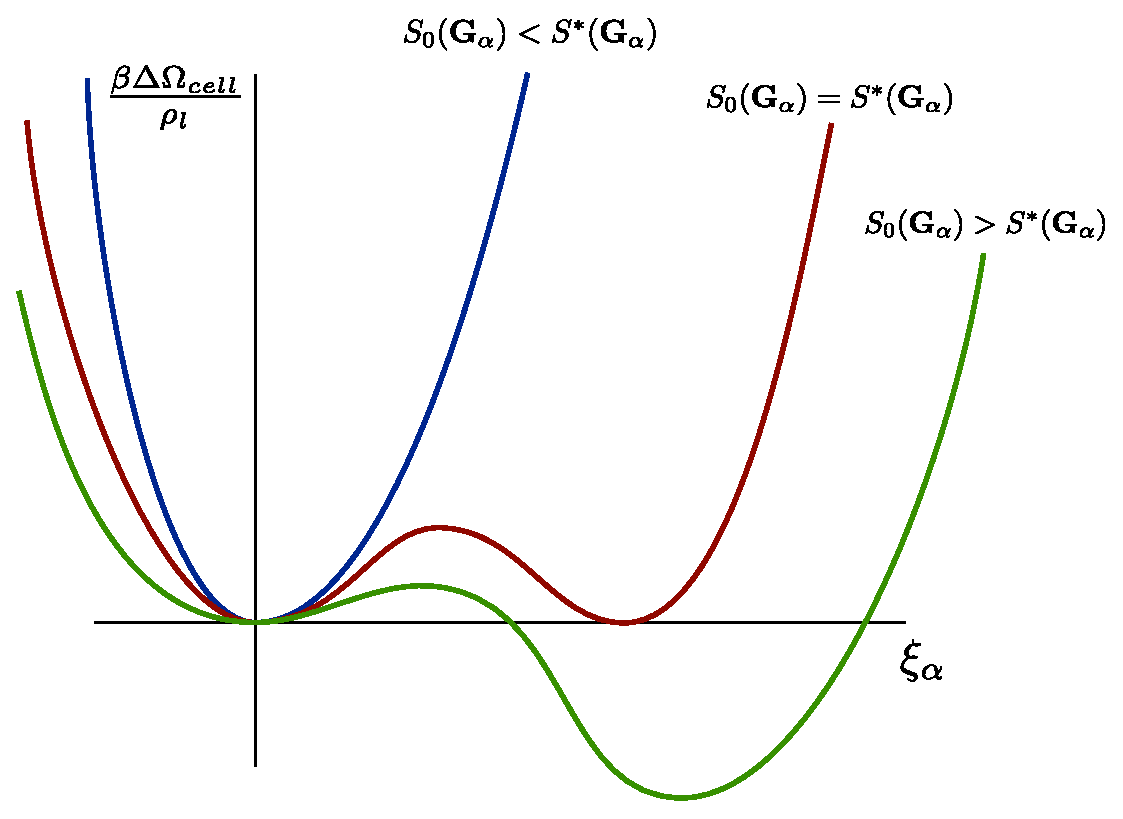
\includegraphics[scale=0.6]{amplitude_transition.eps}
    \caption[Grand Potential through the Solidification transition]{ 
        Schematic view of the grand potential $\beta\Delta\Omega / \rho_l$
        projected on to the $\xi_\alpha$ axis for a three different reference
        structure factors. To minimize the grand potential, finite $\xi_\alpha$
        is stable once $S_0(\mathbf{G}_\alpha) > S^*(\mathbf{G}_\alpha)$
    }\label{fig:amplitude_transition}
\end{figure}
%
Furthermore, equation \ref{amplitude_gp} suggests that the set of critical
structure factors, $\lbrace S^*(\mathbf{G}_\alpha)\rbrace_\alpha$ are material
independent as free parameters remain in the grand potential.
As a consequence, once we specify the symmetry of the lattice a liquid will
solidify into (eg. face-centred-cubic), all materials that undergo this
transition should share these parameters at the melting point. 

Early numerical evidence of this result was supplied by the Hansen-Verlet
criterion \cite{HANSEN69} which states that for Lennard-Jones fluid the peak
of the structure factor is constant along the melting curve with a value 
$\approx 2.85$. It has been noted that in aggregating experimental evidence
many liquids solidifying to fcc structure have a peak value close to 2.8 
whereas those solidifying into bcc structures have a peak value around 3.0
\cite{RAMAKRISHNAN79}.

At this level, the CDFT theory of solidification is an infinite order
parameter theory of solidification. We can simplify the theory by truncating
the number of amplitudes we keep in our expansion of the density. This is
justified by noting that only a few reciprocal lattice families contain the
majority of the grand potential energy of solidification. As seen in table
\ref{table:ramakrishnan_argon} and table \ref{table:ramakrishnan_sodium}
theoretical results from a single amplitude theory (theory I in the results)
are poor but improve significantly with two order parameters (theory II) or
higher order expansions of the free energy (theory III).

\begin{table}[H]
    \begin{subtable}{0.4\linewidth}
        \centering
        \begin{tabular}{l c c c}
            \hline 
            Theory & $\tilde{C}(\mathbf{G}_{[111]})$ & $\tilde{C}(\mathbf{G}_{[311]})$ & $\bar{n}$ \\ 
            \hline
            I & 0.95 & 0.0 & 0.074 \\
            II & 0.65 & 0.23 & 0.270 \\
            III & 0.65 & 0.23 & 0.166 \\
            Experiment & 0.65 & 0.23 & 0.148\\
            \hline
        \end{tabular}
        \caption[Freezing parameters for Argon]{Freezing parameters for fcc with
            comparison to Argon experimental results.
        }\label{table:ramakrishnan_argon}
    \end{subtable}
    \hspace{0.10\linewidth}
    \begin{subtable}{0.4\linewidth}
        \centering
        \begin{tabular}{l c c c}
            \hline 
            Theory & $\tilde{C}(\mathbf{G}_{[110]})$ & $\tilde{C}(\mathbf{G}_{[211]})$ & $\bar{n}$ \\ 
            \hline
            I           & 0.69 & 0.00 & 0.048 \\
            II          & 0.63 & 0.07 & 0.052 \\
            III         & 0.67 & 0.13 & 0.029 \\
            Experiment  & 0.65 & 0.23 & 0.148\\
            \hline
        \end{tabular}
        \caption[Freezing parameters for Sodium]{Freezing parameter for bcc with 
            comparison to Sodium experimental results.
        }\label{table:ramakrishnan_sodium}
    \end{subtable}
    \caption[Table of Ramakrishnan results]{Freezing parameters for fcc and
        bcc systems and comparison to experiment from \cite{RAMAKRISHNAN79}.
        Theory I uses one order parameter, theory II uses two order parameter
        and theory III uses two order parameters with a higher (third) order
        expansion in the free energy. $\eta$ is the fraction density change of
        solidification from equation \ref{eq:eta_def}
    }
\end{table}

%%%%%%%%%%%%%%%%%%%%%%%%%%%%%%%%%%%%%%%%%%%%%
\section{Dynamic Density Functional Theory} %
%%%%%%%%%%%%%%%%%%%%%%%%%%%%%%%%%%%%%%%%%%%%%

In spite of its successes the CDFT theory of solidification cannot be a general
description of solidification as many materials never fully reach equilibrium.
The resulting microstructure affects the mechanical properties of the solid. In
order to improve our theory we need to examine the pathway systems take to
equilibrium so we can understand these microstructural features. We begin with
a brief overview of non-equilibrium statistical mechanics.

%%%%%%%%%%%%%%%%%%%%%%%%%%%%%%%%%%%%%%%%%%%%%%%%%%%%%%%%%%%%%%%%
\subsection{Overview of Non-equilibrium Statistical Mechanics} %
%%%%%%%%%%%%%%%%%%%%%%%%%%%%%%%%%%%%%%%%%%%%%%%%%%%%%%%%%%%%%%%%

Consider a non-equilibrium probability distribution over phase space, $f(\q,
\p; t)$. As a function over phase space, its equation of motion is a simple
result of classical mechanics,
%
\begin{equation}
    \label{cm} 
    \f{d f}{dt} = \l\lbrace f, \mathcal{H} \r\rbrace + \f{\partial f}{\partial t}.
\end{equation}
%
Where, $\l\lbrace \cdot, \cdot \r\rbrace$, denotes the Poisson bracket,
%
\begin{equation}
    \l\lbrace f, g \r\rbrace = \sum_{i = 0}^N \f{\partial f}{\partial q_i}
        \f{\partial g}{\partial p_i} - \f{\partial g}{\partial q_i}
        \f{\partial f}{\partial p_i}.
\end{equation}
%
Of course, the distribution must remain normalized in time and therefore the 
total time derivative must be zero,
%
\begin{equation}
    \int d\q d\p\, f(\q, \p; t) = 1 \rightarrow \f{d f}{dt} = 0.
\end{equation}
%
Accounting for this conservation law in equation \ref{cm}, the resulting
equation of motion is called the \textit{Liouville Equation},
%
\begin{equation}
    \label{liouville} 
    \f{\partial f}{\partial t} = - \l\lbrace f , \mathcal{H} \r\rbrace
\end{equation}
%
Under appropriate conditions the probability distribution, under the action of
the Liouville Equation, will decay to a stable fixed point $f_{eq}(\q, \p)$ we
call equilibrium,
%
\begin{equation}
    \lim_{t \rightarrow \infty} f(\q, \p; t) = f_{eq}(\q, \p)
\end{equation}
%

Using the non-equilibrium probability distribution, we can also discuss
non-equilibrium averages of the density profile and their associated equations
of motions. The non-equilibrium density is written in analogy with equation
\ref{mean_density} by taking of the classical trace of the density operator
over with the non-equilibrium distribution,
%
\begin{equation}
    \rho(x, t) = \mean{\hat{\rho}(x; \q)}_{ne} =
        \trace{\hat{\rho}(x; \q) f(\q, \p, t)}.
\end{equation}
%
Where, $\mean{\cdot}_{ne}$, denotes the non-equilibrium average. Just as the
non-equilibrium probability distribution is driven to equilibrium by the
Liouville Equation, so too is the density profile by its own equation of
motion.

%%%%%%%%%%%%%%%%%%%%%%%%%%%%%%%%%%
\subsection{Equations of Motion} %
%%%%%%%%%%%%%%%%%%%%%%%%%%%%%%%%%%

A variety of equations of motion for the density field are known.  For
instance, we can consider the Navier-Stokes equations of hydrodynamics as one
such equation of motion. If we restrict ourselves to diffusion limited
circumstances, we may derive a much simplier equation of motion. To acheive
this result we use the projection operator method, and assume that the 
density operator is the only relevant variable. Quoting the result from
\cite{ESPANOL09} we find,
%
\begin{equation}
    \label{eq:mean_eom}
    \f{\partial \rho(r, t)}{\partial t} = 
        \nabla \cdot \l[\integrate{r^\prime} \mathbf{D}(r, r^\prime, t) 
        \cdot \nabla^\prime \f{\d \F[\rho]}{\d \rho(r^\prime, t)}\r],
\end{equation}
%
Where, $\mathbf{D}(r, r^\prime, t)$, is the diffusion tensor,
%
\begin{equation}
    \mathbf{D}(r, r^\prime, t) = \int_0^\infty \mathrm{d}\tau^\prime\,
        \trace{f(\q, \p, t)\hat{\mathbf{J}}(r, 0)
        \hat{\mathbf{J}}(r^\prime, \tau^\prime)},
\end{equation}
%
in which $\hat{\mathbf{J}}(r, t)$ is the density flux is,
%
\begin{equation}
    \hat{\mathbf{J}}(r, t) \equiv 
        \sum_i^N \frac{p_i}{m_i} \d(r - q_i).
\end{equation}
%
Theories using equation \label{eq:main_eom} and variations there of are
often called \textit{Dynamic Density Functional Theories} (DDFT) or at times
\textit{Time Dependent Density Functional Theories} (TDDFT) though we will
use the former throughout this work.

The non-equilibrium diffusion tensor presents a significant impedement to
integrating this equation of motion so in practice the diffusion tensor is
often approximated. Following \cite{ESPANOL09}, if we assume that the positions
evolve more slowly than the velocities and that the momenta of different
particles are uncorrelated we can dramatically simplify the diffusion tensor,
%
\begin{equation}
    D(r, r^\prime) = D_0\mathbb{1}\rho(r, t)\d(r - r^\prime).
\end{equation}
%
Where $D_0$ is diffusion coefficient,
%
\begin{equation}
    D_0 = \f{1}{3 m^2} \int_0^\infty \mathrm{d}t 
        \trace{f(\q, \p, t) p_i \cdot p_i(t)}.
\end{equation}
%
Substituting into equation \ref{eq:mean_eom} we find a simplified equation of
motion originally suggested by \cite{MT1999},
%
\begin{equation}
    \label{eq:marconi_eom}
    \f{\partial \rho(r, t)}{\partial t} = 
        \nabla \cdot \l[ D_0 \rho(r, t)
        \nabla \f{\d \F[\rho]}{\d \rho(r, t)}\r].
\end{equation}
%

The equation of motion can also be written as a Langevin equation. In this
variant the equation of motion is for the density \textit{operator},
$\hat{\rho}$, and the noise is assumed to obey a generalized Einstein relation,
%
\begin{gather}
    \label{eq:langevin_eom}
    \f{\partial \hat{\rho}(x, t)}{\partial t} =
        \nabla \cdot \l[
            D_0 \hat{\rho}(x, t) \nabla \l(
            \f{\d \F[\hat{\rho}]}{\d \hat{\rho}}\r)
            \r] + \xi(x, t), \\
    \mean{\xi(x, t)} = 0, \\
    \mean{\xi(x, t)\xi(x^\prime, t^\prime)} = 
        -2 \nabla \cdot \l[ D_0 \rho(x,t) 
            \nabla \d(x - x^\prime) \d(t - t^\prime)\r].
\end{gather}
%
See Appendix \ref{noise} for more details on generalized Einstein relations and
\cite{AR2004} for a detailed discussion about equations \ref{eq:marconi_eom}
and \ref{eq:langevin_eom}.

At times the diffusion tensor is assumed to be constant. This is common place
in many Phase Field Crystal theories. In light of equation
\ref{eq:marconi_eom}, this is akin to assuming the density variations are
small.

Unfortunately, if we were to use the approximate free energy functional
established in equation \ref{cdft_free_energy} in the dynamic density
functional theory of equation \ref{eq:marconi_eom} or \ref{eq:langevin_eom} we
would face a major impedement: the solid state solutions of the density
functional theory approach yield sharply peaked solutions at the position of
the atoms in the lattice. While this is realistic, they are a major challenge
for numerical algorithms. The challenges are two-fold. First, these sharp peaks
require a fine mesh to be resolved resulting in large memory requirement to
simulate domains of any non-trivial scale. Second, lineary stability analysis
of most algorithms demonostrates that the time step size is a monotonic
increasing function of the grid spacing so only small time steps can be taken
on a fine mesh.

One pragmatic solution to this problem is to further approximate the free
energy functional of equation \ref{cdft_free_energy} in such a way as to
produce a theory that retains the essential physics of solidification but
produces a solid state that is more smoothly peaked. As we will see next,
the Phase Field Crystal (PFC) theory acheives precisely this balance.

%%%%%%%%%%%%%%%%%%%%%%%%%%%%%%%%%%%%%%
\section{Phase Field Crystal Theory} %
%%%%%%%%%%%%%%%%%%%%%%%%%%%%%%%%%%%%%%

The phase field crystal theory (PFC) presents a solution to the numerical
difficulties faced by DDFT methods by approximating the free energy in such a
way as to retain the basic features of the theory with a smoother solid state
solution. Starting with the approximate free energy functional of equation
\ref{cdft_free_energy} we proceed as previously by scaling out a factor of the
reference density and changing variables to a dimensionless density $n(r) =
(\rho(r) - \rho_l) / \rho_l$,
%
\begin{equation}
    \f{\beta \F[n(r)]}{\rho_l} = 
        \int dr \l\lbrace (n(r) + 1) \ln( n(r) + 1) - (1 - \beta\mu)n(r) \r\rbrace
        - \f{1}{2} n(r) \ast \rho_l C^{(2)}_0(r, r^\prime) \ast n(r^\prime).
\end{equation}
%
We then Taylor expand the logarithm about the reference density or equivalently
$n(r) = 0$, to fourth order,
%
\begin{equation}
    \label{pfc_free_energy} 
    \f{\beta \F[n(r)]}{\rho_l} =
        \int dr \l\lbrace \f{n(r)^2}{2} - \f{n(r)^3}{6} + \f{n(r)^4}{12} \r\rbrace
        -\f{1}{2} n(r) \ast \rho_l C^{(2)}_0(r, r^\prime) \ast n(r^\prime).
\end{equation}
%
Where the linear term has been dropped because it leaves the equations of
motion invariant.  Most phase field crystal theories also use a simplified
equation of motion as well,
%
\begin{equation}
    \label{pfc_eom}
    \f{\partial n(r, t)}{\partial t} = M \nabla^2 \l(\f{\d \F[n(r)]}{\d n(r)}\r).
\end{equation}
%


\chapter{Simplified Binary Phase Field Crystal Models}
In this chapter we will walk through three simplified binary PFC models. The
first is the original binary PFC model, which, while highly successful at
modelling a few important phenomena is ultimately limited in scope. The second
is the binary structural phase field crystal, or binary XPFC which was
successful in modelling a broad spectrum of crystalline structures, but was
limited in its ability of model liquid instablilities and a variety of phase
diagrams. Finally, we'll see a new contribution to which we will call the
regular phase field crystal model which is successful in modeling a broad
spectrum of invariant binary reactions and crystalline structures. 

\section{Original Binary Phase Field Crystal Model}



\section{Binary Structural Phase Field Crystal Model}

\section{Regular Phase Field Crystal Model}

\section*{Derivation of the General Binary XPFC Free Energy}

Now that we've seen the recipe for building a phase-field crystal theory for a
single component system the process for building a multicomponent theory
proceeds analogously with a few minor changes in perspective.  We start again
by looking at the ideal and excess contributions to the free energy.

\subsubsection{Ideal Free Energy to Two Components} The kinetic energy terms of
each species in the Hamiltonian give rise to seperate contributions to the free
energy as you might expect.  We'll label the two species A and B.

\begin{equation} \beta\F^{tot}_{id}[\rho_A, \rho_B] = \beta\F_{id}[\rho_A] +
\beta\F_{id}[\rho_B] \end{equation} Where,
\begin{description}[labelindent=10pt, labelsep=10pt] \item[$\beta\F_{id}$] is
            the same ideal free energy functional as previously
\end{description}

\subsubsection{Excess Free Energy of a Two Component System} Our expansion of
the excess free energy works just as before but we must sum over the
contributions from each species.

\begin{equation} \beta\F_{ex} = \beta\F_{ex}^0 - \int \,dr C^{(1)}_{i}(r)
\Delta\rho_i(r) - \f{1}{2} \int dr \int dr^\prime \Delta\rho_i(r)
C^{(2)}_{ij}(r, r^\prime) \Delta\rho_j(r^\prime) \end{equation}

Where indices denote species (A or B) and repeated indices are summed over.

\subsubsection{Total free energy of a Two Component System}

Putting together the excess and ideal terms together and dropping the constant
and linear terms as we did previously we find the following total free energy,

\begin{equation} \beta\F[\rho_A, \rho_B] = \int dr \l\lbrace \Delta\rho_i
\ln\l(\f{\Delta\rho_i}{\rho_{i0}}\r) - \Delta\rho_i\r\rbrace - \f{1}{2} \int dr
\int dr^\prime \Delta\rho_i(r) C^{(2)}_{ij}(r, r^\prime) \Delta
\rho_j(r^\prime) \end{equation}

\subsubsection{Changing variables} Typically, the concentration is the variable
we care about in binary systems so instead of preceeding with the usual phase
field crystal approximations at this point we make a change of variables to
concentration, $c$, and total density, $\rho$.

\begin{align} \rho &= \rho_A + \rho_B             & \rho_0 &= \rho_{0A} +
\rho_{0B} \nonumber \\ c &= \f{\rho_A}{\rho_A + \rho_B}    &  c_0 &=
\f{\rho_{0A}}{\rho_{0A} + \rho_{0B}} \nonumber \end{align}

Making this change of variables and seperating total density and concentration
contribution we find a free energy functional of the form,

\begin{equation} \beta\F[c, \rho] = \end{equation}


\chapter{Applications}
\label{chapter:applications}

In this chapter we discuss applications of our improvements to the binary XPFC
model.  To begin we'll discuss a phenomenological equation of motion for the
binary XPFC system. Next we'll examine the process of diffusion limited
precipitation from solution.  Recent experimental work on the precipitation of
gold and silver nanoparticles\cite{LOH17} and on the precipitation of calcium
carbonate \cite{WALLACE13} has demonstrated that pathway to nucleation can
deviate highly from the approximations of Classical Nucleation Theory (CNT).
Both experiments observe spinodal decomposition of the solution prior to
nucleation in the solute rich phase. We'll present early findings that
reproduce this behaviour and additionally show that the growth behaviour post
nucleation may be more complex than usual diffusive growth and coarsening
typically observed. To conclude we discuss future applications both in the
study of precipitation and other areas.

%%%%%%%%%%%%%%%%%%%%%%%
\subsection{Dynamics} %
%%%%%%%%%%%%%%%%%%%%%%%

To examine applications of our improvements to the XPFC model we begin by
considering equations of motion. Following \cite{GREENWOOD11_BINARY}, we use
conservative dynamics for both $n(x, t)$ and $c(x, t)$.
%
\begin{gather}
    \f{\partial n(x, t)}{\partial t} = 
        M_n \nabla^2\l(\f{\d \beta \Delta\F / \rho_0}{\d n(x, t)}\r) 
        + \xi_n(x, t), \\ 
    \f{\partial c(x, t)}{\partial t} = 
        M_c \nabla^2\l(\f{\d \beta \Delta \F / \rho_0}{\d c(x, t)}\r)
        + \xi_c(x, t).
\end{gather}
%
These equations of motion are largely phenomenological as, strictly speaking,
there is no reason that the local concentration should be conserved.  This
conservation can be justified in the limit that the total density does not
deviate far from the reference. When this is the case we have $c \equiv \B /
\rho \approx \B / \rho_0$ which \textit{is} conserved.

%%%%%%%%%%%%%%%%%%%%%%%%%%%%%%%%%%%%%%%%%%%%%%%%%%%%%%%%%%%%%
\section{Multi-step Nucleation of Nanoparticles in Solution} %
%%%%%%%%%%%%%%%%%%%%%%%%%%%%%%%%%%%%%%%%%%%%%%%%%%%%%%%%%%%%%

% Supply some background on the problem and motivation

As stated previously, recent experimental work has shown that precipitation
solution can follow a pathway vary different from that assumed by Classical
Nucleation Theory (CNT)\cite{LOH17, WALLACE13}. CNT assumes that, for binary
systems, assumes that changes in order and composition occur simultaneously. In
contrast, these findings show that in certain systems changes in composition
can precede changes in order via spinodal decomposition.

While there is some dispute about whether or not to call this process a
non-classical \textit{nucleation} pathway \cite{DAVEY13, GEBAUER11}, the
observed pathway to precipitation raises several questions regardless of
semantics about its classification. Many nanoparticle solutions are formed
by precipitation from solution and their size distribution (polydispersity
index) is of key importance to their application. Therefore, a precise
understanding of the kinetic pathway of precipitation is of crucial importance
in designing synthesis techniques of highly mono-disperse nanoparticles.

%%%%%%%%%%%%%%%%%%%%%%%%%%%%%%%%%%%%%%%%%%%%%%%%%%%%%%%%%%%%%%
\subsection{Classical and Non-classical Nucleation Theories} %
%%%%%%%%%%%%%%%%%%%%%%%%%%%%%%%%%%%%%%%%%%%%%%%%%%%%%%%%%%%%%%

% Discuss classical nucleation theory

In CNT, the rate of formation of post-critical can be written as an Arrhenius
equation,
%
\begin{equation}
    J = \f{\partial n^*}{\partial t} = A e^{-\beta\Delta G^{\ddagger}},
\end{equation}
Where,
\begin{description}[labelwidth=1cm, align=right]
    \item[$A$] is a constant prefactor,
    \item[$\Delta G^\ddagger$] is the Gibbs free energy of a critical nucleus
    and, 
    \item[$n^*$] is the number if critical nuclei.
\end{description}
% 
Following \cite{MYERSON04}, the probability of nucleation in droplet of volume
$V$ is then,
%
\begin{equation}
    f_{nuc}(t) = \mean{\f{N_{liq}}{N_{total}}} = e^{-J V t}.
\end{equation}

% Discuss non-classical nucleation theory and the methods of reaction co-ordinates

CNT assumes that there is a single critical state which is specified by the
thermodynamic parameters of the target phase at a critical radius $R^*$. This
naive approach dramatically underestimate the time required to assemble a
critical nucleus due to its simplistic parametrization of the kinetic pathway
\cite{LUTSKO15, MYERSON04, MYERSON09}.

Improvements can be made to the model by increasing the parameter space.
Considering radius and density \cite{LUTSKO15} gives good agreement with
nucleation of globular proteins, for example. One problem with this approach is
the selection of appropriate parameters. There is no guarantee that a finite
set parameters will describe the kinetic pathway taken by a nucleus and if we
are without a fundamental technique for calculating the chosen parameters we
have little way of knowing if our theory is accurate or simply over-fit. In
\cite{MYERSON09}, for example, nucleation data is fit to the functional form
instead of using calculated or otherwise measured parameters.

% Posit that field theory present an unbiased (un-parameterized) approach to nucleation

Statistical field theories such as the XPFC model provide an answer to this
problem by taking a unbiased approach to nucleation. The critical state, and
entire kinetic pathway, can be examined with any parametrization. The equations
of motion can be integrated numerically for an ensemble systems and nucleation
details measured from the results. Unlike other numerical approaches to
nucleation like molecular dynamics or density functional theory the PFC model
can examine nucleation on diffusive time scales.

%%%%%%%%%%%%%%%%%%%%%%%%%%%%%%%%%%%%%%
\subsection{Modelling Precipitation} %
%%%%%%%%%%%%%%%%%%%%%%%%%%%%%%%%%%%%%%

% Motivate a submerged spinodal phase diagram

To construct an appropriate free energy functional for this system we consider
the structure of its equilibrium phase diagram. Precipitation is indicative of
a simple liquid-solid coexistance curve. The presence of spinodal decomposition
under certain circumstances indicates that is a metastable liquid spinodal
submerged beneath the liquid-solid coexistance curve \cite{DAVEY13}. We assume
that there must exist conditions under which the spinodal decomposition of the
metastable liquid phase occurs more rapidly than nucleation directly from
solution (ie., classical nucleation).

% Discuss the implementation of this phase diagram using our improvements

Producing a phase diagram with these characteristics is very similar to
modelling a monotectic system with the exception that the spinodal temperature
$T_c$ must be low enough to hide the entire liquid spinodal below the
coexistance curve.  We will also centre the interpolation function $\zeta_c$
about the $c = 1$ point so that the concentration is interpreted as the solute
concentration. The resulting density-density correlation function for a 2
dimensional hexagonal precipitate would be,
%
\begin{equation}
    \label{eq:precip_corr}
    \tilde{C}_{nn}(k; c) = \exp\l\lbrace - \f{(c - 1)^2}{2\sigma_c^2}\r\rbrace
        \exp\l\lbrace \f{T}{T_0} \r\rbrace 
        \exp\l\lbrace - \f{(k - k_{10})^2}{2\sigma^2} \r\rbrace,
\end{equation}
%
Where,
\begin{description}[labelwidth=1cm, align=right]
    \item[$\sigma_c$] is the width of the interpolation function $\zeta(c)$
        which controls the solvent solubility in the precipitate in this case
        and,
    \item[$k_{10}$] is the length of the [10] reciprocal lattice vector of the
        preciptate in equilibrium.
\end{description}

An example of a system with appropriate parameters can be seen in figure
\ref{fig:precip_phase_dia}. The metastable binodal (coexistance) and spinodal
curves are depicted below the coexistance curve.

\begin{figure}
    \centering	
    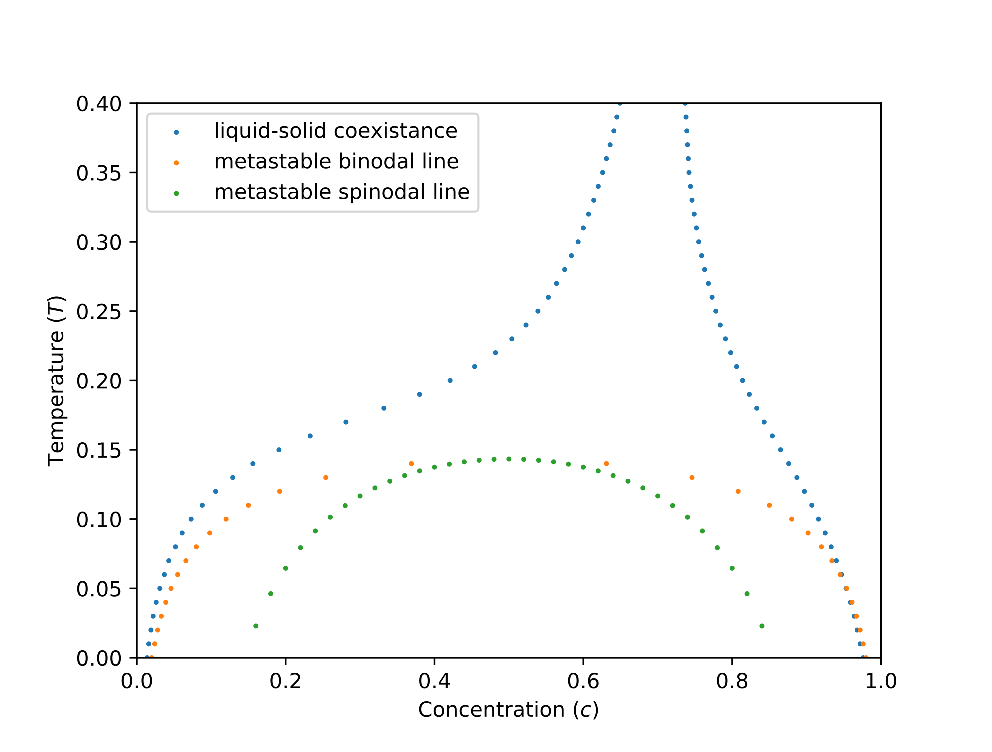
\includegraphics[scale=0.8]{solution.eps}
    \caption[Coexistance Phase Diagram with Metastable Spinodal]{
        \label{fig:precip_phase_dia} Phase Diagram of a Precipitating Solution
        with hexagonal $\alpha$ phase. The free energy parameters are $\eta =
        2$, $\chi = 1$, $\omega=0.3$, $\epsilon_0=30$, $T_c = 0.15$ and
        $c_0=0.5$. The parameters for the correlation function from equation
        \ref{eq:precip_corr} are $\sigma = 0.8$, $k_{10} = 2\pi$, $T\_0 = 1$
        and $\sigma_c = 0.5$.
    }
\end{figure}

%%%%%%%%%%%%%%%%%%%%%%%%%%%%%%%%%%%%%
\subsection{Results and Discussion} %
%%%%%%%%%%%%%%%%%%%%%%%%%%%%%%%%%%%%%

% Describe with supporting figures the typical path way of precipitation.

Using the system with phase diagram depicted in figure
\ref{fig:precip_phase_dia}, we examine the precipitation process under a quench
the passes the metastable spinodal curve. The spinodal curve marks an inflection
point in the liquid free energy meaning the metastable liquid becomes fully
unstable and decomposes as a result. A typical quench from a uniform solution
of $c = 0.3$ to $T = 0.07$ is depicted in figure \ref{fig:precipitation}. We
can clearly see that nucleation is preceded by spinodal decomposition as in
experimental the experimental findings. 
%
\begin{figure}
    \centering
    \begin{subfigure}[b]{0.3\textwidth}
        
\includegraphics[width=\textwidth]{initial}
        \label{fig:initial}
        \caption{}
    \end{subfigure}
    ~
    \begin{subfigure}[b]{0.3\textwidth}
        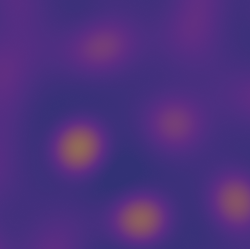
\includegraphics[width=\textwidth]{early_spinodal}
        \label{fig:early_spinodal}
        \caption{}
    \end{subfigure}
    ~
    \begin{subfigure}[b]{0.3\textwidth}
        
\includegraphics[width=\textwidth]{devel_spinodal.png}
        \label{fig:devel_spinodal}
        \caption{}
    \end{subfigure}

    \vspace{0.25cm}
    \begin{subfigure}[b]{0.3\textwidth}
        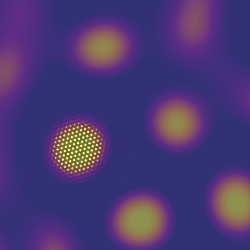
\includegraphics[width=\textwidth]{nucleation}
        \label{fig:nucleation}
        \caption{}
    \end{subfigure}
    ~
    \begin{subfigure}[b]{0.3\textwidth}
        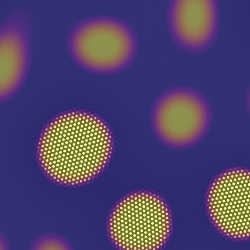
\includegraphics[width=\textwidth]{nucleation_and_sacrificial_growth}
        \label{fig:nucleation_and_growth}
        \caption{} 
    \end{subfigure}
    ~
    \begin{subfigure}[b]{0.3\textwidth}
        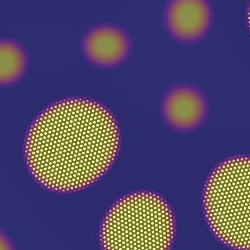
\includegraphics[width=\textwidth]{sacrificalgrowth}
        \label{fig:sacrifical_growth}
        \caption{}
    \end{subfigure}
    
    \vspace{0.25cm}
    \begin{subfigure}[b]{0.3\textwidth}
        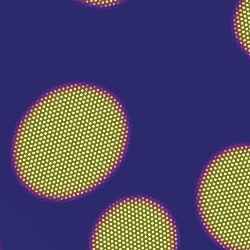
\includegraphics[width=\textwidth]{crystalgrowth}
        \label{fig:crystalgrowth}
        \caption{}
    \end{subfigure}
    ~
    \begin{subfigure}[b]{0.3\textwidth}
        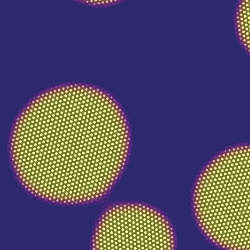
\includegraphics[width=\textwidth]{crystalgrowth2}
        \label{fig:crystalgrowth2}
        \caption{}
    \end{subfigure}
    ~ 
    \begin{subfigure}[b]{0.3\textwidth}
        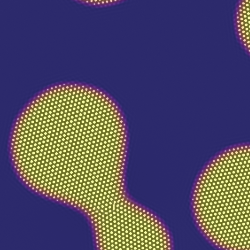
\includegraphics[width=\textwidth]{crystalgrowth3}
        \label{fig:crystalgrowth3}
        \caption{}
    \end{subfigure}
    \caption[Stages of precipitation of nanoparticles from solution]{
        \label{fig:precipitation}
        Various stages of precipitation of nanoparticles from solution. All
        thermodynamic parameters are shared with figure
        \ref{fig:precip_phase_dia}. The initial condition is a uniform solution
        quenched abruptly to $T$ = 0.07. The initial condition has
        concentration $c = 0.3$ and relative density $n = 0.05$. Mobilities
        $M_n$ and $M_c$ are set to 1 and $W_c$ is set to 3.0. Numerical
        parameters are grid spacing $\Delta x = 0.125$ on a 1024 by 1024
        lattice with time step size $\Delta t = 0.0025$. Sub-figures (a) - (c)
        show spinodal decomposition of the liquid into solute right and solute
        poor regions. Sub-figures (d) - (f) show nucleation of the solid and
        solid growth at the expense of liquid regions.  The remaining
        sub-figures show only nanoparticle growth and coarsening.
    }
\end{figure}
%
We also see that once any solute-rich regions crystallize, their growth is
accelerated at the expense of uncrystallized solute-rich regions. We call this
phenomena \textit{sacrificial growth}. 
%
% Discuss the growth picture (hyper / hypo diffusive)
%
To quantify this phenomena we examine the mean radius $\mean{R(t)}$ of
solute-rich domains in time of an ensemble of 120 quenches. Here we define the
mean radius as the square root of the mean area,
%
\begin{equation}
    \mean{R(t)} = \sqrt{\mean{A(t)}}.
\end{equation}
%
In purely diffusive growth the mean radius should scale as $\mean{R(t)} \sim
t^{1/2}$ and coarsen (the very late stages of growth) as $\mean{R(t)} \sim
t^{1/3}$. In figure \ref{fig:scaling} we plot the growth exponents in time on a
log-log plot with diffusive growth marked in black for reference. Indeed for
early crystalline regions we see hyper-diffusive growth which decays to
hypo-diffusive after uncrystallized regions have disappeared.
%
\begin{figure}
    \centering
    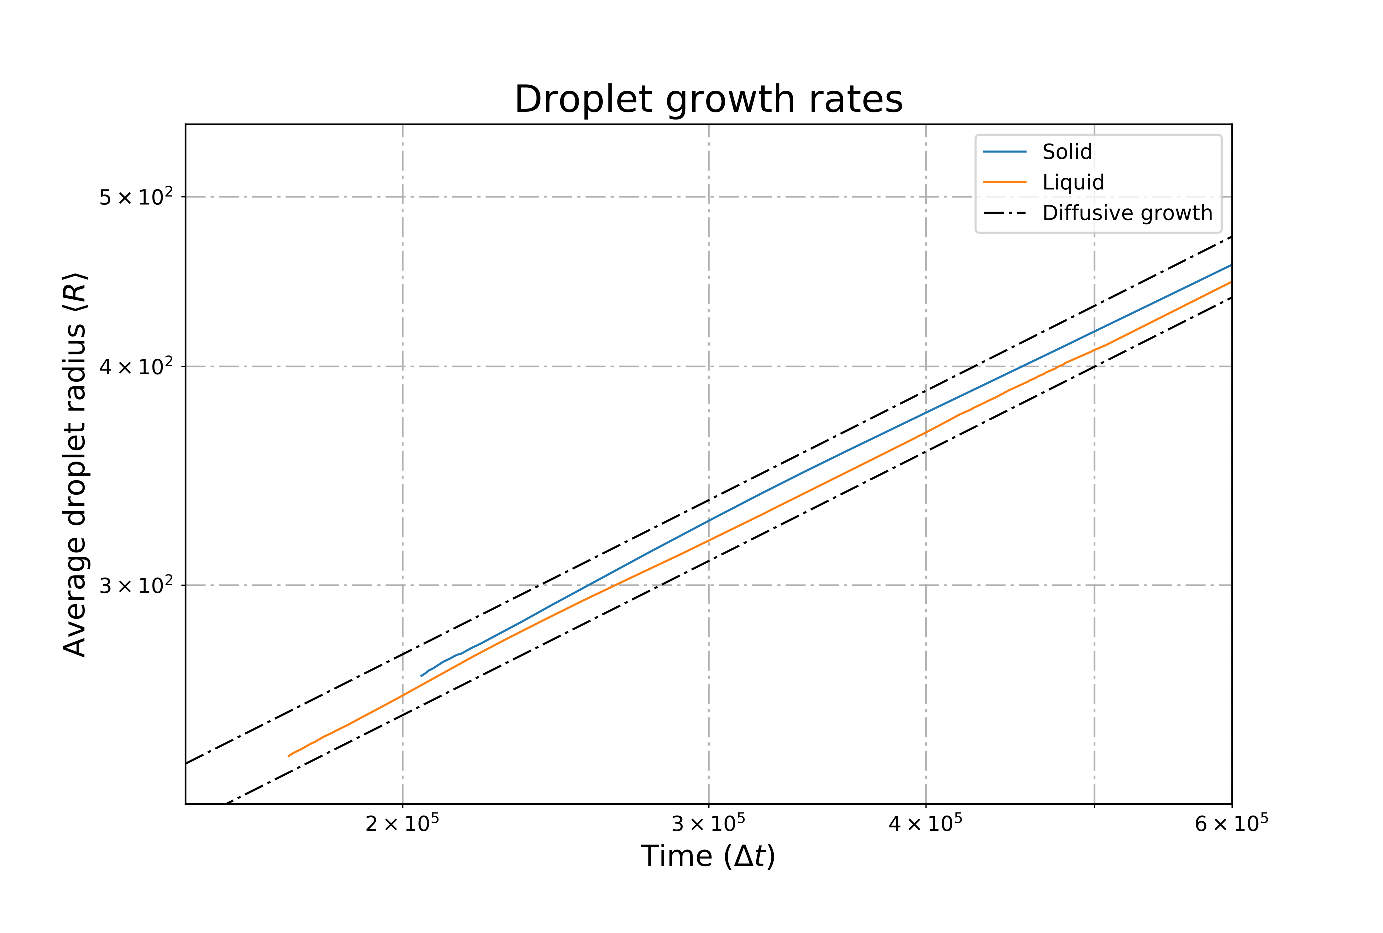
\includegraphics[width=\textwidth]{scaling}
    \caption{
        \label{fig:scaling}
        Droplet growth exponents
    }
\end{figure}

% Discuss the nucleation picture (fraction of uncrystallized droplets)
% and compare with MYERSON for example

During sacrificial growth we see that nucleation is suppressed in the remaining
uncrystallized solute-rich regions. When both crystallized and uncrystallized
solute-rich regions exist, solute is segregated into crystallized regions
because of the difference in chemical potential. Constricted by surface tension
and deprived of solute, these remaining droplets have a far slower nucleation
rate than when no crystallized regions exist. This can be seen more
quantitatively by examining the fraction of uncrystallized droplets in time as
in figure \ref{fig:incubation}. At $\sim 50\%$ crystallization we see a
pronounced reduction in the nucleation rate as the diffusive process of
sacrificial growth dominates.

\begin{figure}
    \centering
    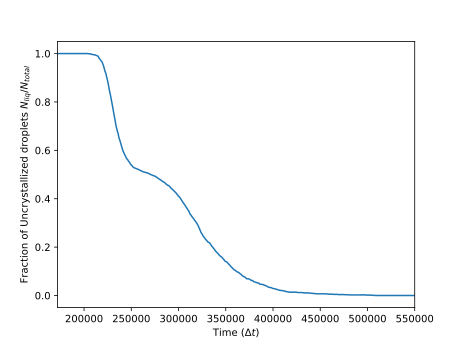
\includegraphics[width=0.7\textwidth]{incubation}
    \caption[Fraction of uncrystallized droplets in time]{
        \label{fig:incubation}
        Fraction of uncrystallized droplets in time
    }
\end{figure}

%%%%%%%%%%%%%%%%%%%%%%%%%%%%%%%%%%%%%%%%%%%%%%%
\section{Future Applications and Conclusions} %
%%%%%%%%%%%%%%%%%%%%%%%%%%%%%%%%%%%%%%%%%%%%%%%

% Explore the remainder of the phase space of nucleation
% Is CNT valid on some regime?
% Is the turnbull model valid elsewhere?

The works shown here represent the behaviour of quench with a particular set of
parameters, but they point to a richness in the possible pathways to
precipitation. The current view on nucleation is limited in its ability to describe
the sacrificial growth phenomena .....  

% List other applications (stability of nanocrystalline alloys is the top of my
% list)

% Wrap up the thesis complete here? Or in a new "chapter"



%%%%%%%%%%%%%%%%%%%%%
% -- Back Matter -- %
%%%%%%%%%%%%%%%%%%%%%

\appendix

\chapter{Noise in Nonlinear Langevin Equations}
\label{noise}
\label{appendix:noise}
\label{noiseappendix}

When using Langevin equations to study non-equilibrium statistical mechanics,
the noise strength can be linked to the transport coefficients through a
generalization of the Einstein relation. The generalization was first developed
by Onsager and Machlup \cite{OnsagerMachlup}. The typical strategy for deriving
such a relationship is to evaluate the equilibrium pair correlation function by
two separate methods: the equilibrium partition functional and the equation of
motion\footnote{For considerations far from equilibrium see \cite{Lax, Ronis,
Fox_and_Uhlenbeck}}.

While the equilibrium partition functional gives pair correlation through the
typical statistical mechanical calculation, the equation of motion can be used
to derive a dynamic pair correlation function that must be equal to the
equilibrium pair correlation function in the long time limit.

In what follows we'll look at how to formulate a generalized Einstein relation
from a generic Langevin equation and then calculate two specific examples using
Model A dynamics with a $\phi^4$ theory and Time Dependent Density Functional
Theory (TDDFT) with a general Helmholtz free energy.

%%%%%%%%%%%%%%%%%%%%%%%%%%%%%%%%%%%%%%%%%%%%%%%%%%%%%%%%%%%%%%%%
\section{Generalized Einstein Relations in an Arbitrary Model} %
%%%%%%%%%%%%%%%%%%%%%%%%%%%%%%%%%%%%%%%%%%%%%%%%%%%%%%%%%%%%%%%%

We start by considering a set of microscopic observables, $a_i(r, t)$, that are
governed by a nonlinear Langevin equation,
%
\begin{equation} 
    \f{\partial \mathbf{a}(r, t)}{\partial t} = 
        F[\mathbf{a}(r,t)]
      + \boldsymbol{\xi}(r,t).
\end{equation}
%
Where, $\mathbf{a}$, denotes a vector of our fields of interest. These
microscopic equation of motion may have been derived from linear response,
projection operators or some other non-equilibrium formalism. We assume that
the random driving force, $\boldsymbol{\xi}(r, t)$ is unbiased, Gaussian noise
that is uncorrelated in time,
%
\begin{gather}
    \mean{\boldsymbol{\xi}(r,t)} = 0, \\ 
    \label{eq:noise_form} 
    \mean{\boldsymbol{\xi}(r,t) \boldsymbol{\xi}^\dagger(r^\prime,t^\prime)} =
        \mathbf{L}(r, r^\prime)\d(t-t^\prime).
\end{gather}
%
This assumption is justified by positing that the stochastic driving force is
the aggregated affect of many random microscopic processes that satisfy the
central limit theorem so we may assume a Gaussian form. We wish to constrain
the form of the covariance matrix, $\mathbf{L}$, by demanding that the solution
to the Langevin equation eventually decays to equilibrium and that correlations
in equilibrium are given by Boltzmann statistics.

We begin by linearizing the equation of motion about an equilibrium solution,
$\mathbf{a}(r, t) = \mathbf{a}_{eq}(r) + \hat{\mathbf{a}}(r, t)$.
%
\begin{equation}
    \f{\partial \hat{\mathbf{a}} (r, t)}{\partial t} =
        \mathbf{M}(r, r^\prime) \ast \hat{\mathbf{a}}(r^\prime, t) +
\boldsymbol{\xi}(r, t) 
\end{equation}
%
Where, $\ast$ denotes an inner product and integration over the repeated
variable. eg:
%
\begin{equation}
    \mathbf{M}(r, r^\prime)\ast \hat{\mathbf{a}}(r^\prime) =
\sum_j \int\,dr^\prime M_{ij}(r, r^\prime) \hat{a}_j(r^\prime).
\end{equation}
%
We can formally solve our linearized equation of motion,
%
\begin{equation}
    \label{eq:formal_sol}
    \hat{\mathbf{a}}(r, t) = e^{\mathbf{M}(r,
r^\prime)t}\ast\hat{\mathbf{a}}(r^\prime, 0) + \int_0^t d\tau\,
e^{\mathbf{M}(r, r^\prime)(t-\tau)} \ast \boldsymbol{\xi} (r^\prime, \tau),
\end{equation}
%
And use this formal solution to evaluate the dynamic pair correlation function,
%
\begin{align} 
    \label{eq:formal_corr}
    \mean{\hat{\mathbf{a}}(r,t)\hat{\mathbf{a}}^\dagger(r^\prime, t^\prime)} &=
             e^{\mathbf{M}(r, r_1)t}
        \ast \mean{\hat{\mathbf{a}}(r_1, 0)\hat{\mathbf{a}}^\dagger(r_2, 0)}
        \ast e^{\mathbf{M}^\dagger(r^\prime, r_2)t^\prime} \nonumber \\ 
     &+ \int_0^t \int_0^{t^\prime}d\tau d\tau^\prime\, 
        e^{\mathbf{M}(r, r_1)(t-\tau)} 
        \ast \mean{ \boldsymbol{\xi}(r_1, 0)\boldsymbol{\xi}^\dagger(r_2, 0)}
        \ast e^{\mathbf{M}^\dagger(r^\prime, r_2)(t^\prime-\tau^\prime)}.
\end{align}
%
To evaluate the equilibrium correlation function we take the limit as each time
goes to infinity together ($t = t^\prime \rightarrow \infty$). It is important
to note that every eigenvalue of $\mathbf{M}$ must be negative for our solution
to decay to equilibrium in the long time limit (eg.
$lim_{t\rightarrow\infty}\hat{\mathbf{a}}(r, t) = 0$) and as such the first
term in equation \ref{eq:formal_corr} won't contribute to the equilibrium
pair correlation. This is as we might expect as the first term holds the
contributions to the dynamic correlation function from the initial conditions.
The second term can be evalutated by substituting the noise correlation from
equation \ref{eq:noise_form} and
evaluating the delta function.
%
\begin{equation}
    \mathbf{\Gamma}(r, r^\prime) = \lim_{t\rightarrow\infty}
    \mean{\hat{\mathbf{a}}(r, t)\hat{\mathbf{a}}^\dagger(r^\prime, t)} =
    \int_0^\infty dz \,e^{\mathbf{M}(r, r_1)z}\ast\mathbf{L}(r_1, r_2)\ast
    e^{\mathbf{M}^\dagger(r^\prime, r_2)z}
\end{equation}
%
Considering the product $\mathbf{M}(r, r_1)\ast\mathbf{\Gamma}(r_1, r^\prime)$
and performing an integration by parts yields the final generalized Einstein
relation.
%
\begin{equation}
    \label{eq:generalized_einst} 
    \mathbf{L}(r, r^\prime) = - \l\lbrace
          \mathbf{M}(r, r_1) 
     \ast \mathbf{\Gamma}(r_1, r^\prime) 
        + \mathbf{\Gamma}(r, r_1)
     \ast \mathbf{M}^\dagger(r_1, r^\prime) \r\rbrace
\end{equation}
%

As we can see from equation \ref{eq:generalized_einst}, near equilibrium the
noise correlation function is a simple function of the pair correlation
function, $\mathbf{\Gamma}(r, r^\prime)$ and the linearized transport
coefficient $\mathbf{M}(r, r^\prime)$.

As a simple check we apply our result to the original work of Einstein. Recall
that in the over damped limit the equation of motion for the velocity for a 1
dimensional Brownian particle is,
%
\begin{equation}
    \f{\partial v(t)}{\partial t} = -\gamma v (t) + \xi(t).
\end{equation}
%
This equation is alread linear so we can pick off the linearized transport
coefficient as $-\gamma$. The pair correlation function in equilibrium is given
by equipartition theorem as,
%
\begin{equation}
    \mean{v^2} = \f{k_b T}{m}.
\end{equation}
%
Simply applying equation \ref{eq:generalized_einst} we find,
%
\begin{equation}
    \mean{\xi(t)\xi(t^\prime)} = 2 \f{k_b T \gamma}{m} \d(t - t^\prime),
\end{equation}
%
As expected. Satisfied that equation \ref{eq:generalized_einst} reduces to 
the correct result for the base case we proceed to examine two examples
that are guininely nonlinear field theories.

%%%%%%%%%%%%%%%%%%%%%%%%%%%%%%%
\section{Example 1 - Model A} %
%%%%%%%%%%%%%%%%%%%%%%%%%%%%%%%

As a first nontrivial example of calculating an Einstein relation consider the
following free energy functional under non-conservative, dissipative dynamics.
%
\begin{gather}
    \beta \F[\phi] = \int dr \l\lbrace \f{1}{2}\vert \nabla
    \phi(x) \vert^2 + \f{r}{2}\phi^2(x) + \f{u}{4!}\phi^4(x)  +
    h(x)\phi(x)\right\rbrace \\ \f{\partial \phi(x,t)}{\partial t} = -\Gamma
    \left(\f{\delta \beta \F[\phi]}{\delta \phi(x)}\right) + \xi(x, t)
\end{gather}
%
The random driving force, $\xi$, is Gaussian noise, uncorrelated in time.
%
\begin{align} \l\langle \xi (x, t) \r\rangle &= 0 \\ \l\langle \xi (x, t)
\xi(x^\prime, t^\prime) \r\rangle  &= L(x-x^\prime) \delta (t - t^\prime)
\end{align}
%
To compute the Einstein relation for this theory we start by calculating the
pair correlation function using the equilibrium partition function and
Boltzmann statistics.

\subsection{The partition function route}

In equilibrium the probability of particular field configuration is given by
the Boltzmann distribution.
%
\begin{equation} \mathcal{P}_{eq}[\phi] =
\f{e^{-\beta\F[\phi]}}{\mathcal{Z}[h(x)]} \end{equation}
%
Where, $\mathcal{Z}[h(x)]$ is the partition functional and is given by a path
integral over all field configurations.
%
\begin{equation} \mathcal{Z}[h(x)] = \int \mathcal{D}[\phi] e^{-\beta\F[\phi]}
\end{equation}
%
Evaluation of the partition function is of some importance because it plays the
role of a moment generating function.
%
\begin{equation}\label{gen} \f{1}{\Z[h]}\f{\delta^n \Z[h]}{\delta
h(x_1)...\delta h(x_n)} = \langle \phi(x_1)...\phi(x_n)\rangle \end{equation}
%
In general the partition function cannot be computed directly, but in the
special case of Gaussian free energies it can. To that end we consider
expanding $\phi$ around an equilibrium solution, $\phi(x) = \phi_0 +
\Delta\phi(x)$, and keeping terms to quadratic order in the free energy.
%
\begin{equation} \beta\F[\Delta\phi] = \int dr \,\left\lbrace
\f{1}{2}\Delta\phi(x) \left(r - \nabla^2 + \f{u}{2}\phi_0^2\right)
\Delta\phi(x) - h(x)\Delta\phi(x) \right\rbrace \end{equation}
%
Here the partition function is written in a suggestive form. As stated
previously, functional integrals are difficult to compute in general, but
Gaussian functional integrals do have a solution.

\subsubsection{Computing the Pair correlation function in the Gaussian
approximation}

To compute the pair correlation function we use the Fourier space variant of
the partition function,
%
\begin{equation} 
    \Z[\tilde{h}(k)] \propto \exp\left\lbrace \f{1}{2}\int dk\,
        \f{h(k)h^{*}(k)}{r + \f{u}{2}\phi_0^2 +  \vert k \vert^2}
        \right\rbrace.
\end{equation} 
%
The pair correlation function, $\langle
\Delta\tilde{\phi}(k)\Delta\tilde{\phi}^{*}(k)\rangle$, is then computed using
equation \ref{gen}.
%
\begin{equation} \l\langle \Delta\fphi(k)\Delta\fphi^{*}(k^\prime) \r\rangle =
\f{2\pi \delta(k+k^\prime)}{r + \f{u}{2}\phi_0^2 + \vert k \vert^2}
\end{equation}
%
%%%%%%%%%%%%%%%%%%%%%%%%%%%%%%%%%%%%%%%%%%%
\subsection{The Equation of Motion Route} %
%%%%%%%%%%%%%%%%%%%%%%%%%%%%%%%%%%%%%%%%%%%

The equation of motion supplies a second method for evaluating the pair
correlation function in equilibrium.
%
\begin{equation} \f{\partial \phi}{\partial t} =
-\Gamma\left((r-\nabla^2)\phi(x,t) + \f{u}{3!}\phi^3(x,t)\right) + \xi(x, t),
\end{equation}
%
Our equation of motion, can be linearized around an equilibrium solution,
$\phi_0$, just as we did in the partition function route to the pair
correlation function. In a similar vain, we will Fourier transform the equation
of motion as well.
%
\begin{equation} \f{\partial \Delta\fphi(k, t)}{\partial t} = -\Gamma\left((r +
\f{u}{2}\phi_0 + \vert k \vert^2)\Delta\fphi(k,t)\right) + \xi(x,t)
\end{equation}
%
Comparing with our generalized approach we can read of $M(k, k^\prime)$ from
the lineared equation of motion:
%
\begin{equation} M(k, k^\prime) = -\Gamma\l((r + \f{u}{2}\phi_0 + \vert k
\vert^2)\r)\d(k + k^\prime) \end{equation}
%
Finally, once we compute the generalized Einstein relation with our specific
pair correlation and $M(k, k^\prime)$ we find,
%
\begin{equation} L(k, k^\prime) = 2\Gamma \d(k + k^\prime), \end{equation}

Or equivalently,

\begin{equation} L(x, x^\prime) = 2\Gamma \d(x - x^\prime).  \end{equation}

%%%%%%%%%%%%%%%%%%%%%%%%%%%%%%%%%%%%%%%%%%%%%%%%%%%%%%%%%%%%%%%%
\section{Example 2 - Time Dependent Density Functional Theory} %
%%%%%%%%%%%%%%%%%%%%%%%%%%%%%%%%%%%%%%%%%%%%%%%%%%%%%%%%%%%%%%%%

In time dependent density functional theory (TDDFT) we have an equation of
motion of the following form,

\begin{equation} \f{\partial \rho(r, t)}{\partial t} = D_0 \nabla \cdot
\l[\rho(r,t)\nabla \l(\f{\d \F[\rho]}{\d \rho}\r)\r] + \xi(r, t) \end{equation}
%
Where, $D_0$ is the equilibrium diffusion constant and $\xi$ is the stochastic
driving force. We assume once again that the driving force has no bias, but we
now allow the noise strength to be a generic kernel $L(r, r^\prime)$.
%
\begin{align} \langle \xi(r,t) \rangle &= 0 \\ \l\langle \xi(r, t)
\xi(r^\prime, t^\prime) \r\rangle &= L(r, r^\prime) \d (t -t^\prime)
\end{align}
%
%%%%%%%%%%%%%%%%%%%%%%%%%%%%%%%%%%%%%%%%%%%%%%%%%%%%%%%%%%%%%
\subsection{Pair Correlation from the Partition Functional} %
%%%%%%%%%%%%%%%%%%%%%%%%%%%%%%%%%%%%%%%%%%%%%%%%%%%%%%%%%%%%%

Just like with the $\phi^4$ model we want to expand our free energy functional
around an equilibrium solution. In this case our free energy functional is
generic so this expansion is purely formal.
%
\begin{equation} \F[\rho] = \F_{eq} + \beta\int dr \l(\l.\f{\d \F[\rho]}{\d
\rho(r)}\r)\r\vert_{\rho_{eq}}\Delta\rho(r) + \f{1}{2} \int dr \int dr^\prime
\Delta\rho(r) \l(\l.\f{\d^2 \F[\rho]}{\d \rho(r) \d
\rho(r^\prime)}\r)\r\vert_{\rho_{eq}} \Delta\rho(r^\prime) \end{equation}
%
The first term we can neglect as it adds an overall scale to the partition
function that will not affect any of moments. Second moment only shifts the
average so we can ignore it as well and so we're left with a simple quadratic
free energy once again.
%
\begin{equation} \F[\rho] = \f{1}{2}\int dr \int dr^\prime \Delta \rho(r)
\Gamma^{-1}(r, r^\prime) \Delta \rho(r^\prime) \end{equation}
%
Where, $\Gamma^{-1}(r, r^\prime)$ is the second functional derivative of the
free energy functional in equilibrium. Computing the pair correlation function
from the partition function yields, as might be expected,
%
\begin{equation} \l\langle \Delta\rho(r) \Delta\rho(r^\prime) \r\rangle =
\Gamma(r, r^\prime) \end{equation}
%
%%%%%%%%%%%%%%%%%%%%%%%%%%%%%%%%%%%%%%%%%%%%%%%
\subsection{Linearing the equation of motion} %
%%%%%%%%%%%%%%%%%%%%%%%%%%%%%%%%%%%%%%%%%%%%%%%

Linearizing the equation of motion about an equilibrium solution we find the
following form,
%
\begin{equation} \f{\partial \Delta \rho (r, t)}{\partial t} = D_0\nabla \cdot
\l[\rho_{eq}(r)\nabla \l(\Gamma^{-1}(r, r^\prime)\ast \Delta\rho(r^\prime,
t)\r)\r] + \xi(r, t) \end{equation}
%
Once again we can read of the kernel $M(r, r^\prime)$ from the linearized
equation.
%
\begin{equation} M(r, r\prime) = D_0\nabla \cdot \l[\rho_{eq}(r)\nabla
\l(\Gamma^{-1}(r, r^\prime)\r)\r] \end{equation}
%
Plugging into the generalized Einstein relation, we find a the factors of the
pair correlation cancel giving a simple form for the kernel $L(r, r^\prime)$.
%
\begin{equation} L(r, r^\prime) =
-2D_0\nabla\cdot\l(\rho_{eq}(r)\nabla\r)\delta(r - r^\prime) \end{equation}
%

\nocite{Ronis, Fox_and_Uhlenbeck, Lax}


\chapter{Gaussian Functional Integrals}
\subsubsection{Gaussian Functional Integrals}

In the study of the statistical physics of fields we often encounter functional integrals of the form,

\begin{equation}
\Z[h(x)] = \int \D[\phi] \exp\left\lbrace - \int dx \int dx^\prime \left[ \f{1}{2}\phi(x) \mathbf{K}(x, x^\prime) \phi(x^\prime)\right] +  \int dx \left[h(x) \phi(x)\right]\right\rbrace.
\end{equation}

Solutions to this integral are not only important in there own right but are also the basis perturbative techniques. The detail of how to solve this integral can be found in \cite{Kardar} and are repeated here for the convenience of the reader.

This integral is simply the continuum limit of a multivariable Gaussian integral,

\begin{equation}
\Z[\mathbf{h}] = \int \prod_i dx_i \exp \left\lbrace - \f{1}{2}\sum_i \sum_j x_i\, \mathbf{K}_{ij}\, x_j  + \sum_i h_i x_i\right\rbrace,
\end{equation}
For which the solution is,

\begin{equation}
\Z[\mathbf{h}] = \sqrt{\f{2\pi}{\det(\mathbf{K})}} \exp\left\lbrace \f{1}{2} \sum_i \sum_j h_i \mathbf{K}_{ij}^{-1} h_j\right\rbrace.
\end{equation}
In the continuum limit, the solution has an analogous form.

\begin{equation}\label{part}
\Z[h(x)] \propto \exp\left\lbrace \int dx \int dx^\prime \left[ \f{1}{2}h(x) \mathbf{K}^{-1}(x, x^\prime) h(x^\prime)\right] \right\rbrace
\end{equation}
Where $\mathbf{K}^{-1}$ is defined by,

\begin{equation}
\int dx^\prime \mathbf{K}(x, x^\prime)\mathbf{K}^{-1}(x^\prime, x^{\prime\prime}) = \delta(x - x^{\prime\prime}).
\end{equation}
Ultimately, we don't need to worry about the constant of proportionality in equation \ref{part} because we'll be dividing this contribution when calculating correlation functions.


\chapter{Binary Correlation Functions}
\label{binary_correlations}
\label{appendix:binary_corr}

When developing the binary PFC model we often change variables from $\A$ and
$\B$ to $n$ and $c$.  This change of variable is helpful in identifying the
results of the PFC theory with established results in the field as
concentration and total density are more commonly used in the field of material
science. Computing the bulk terms (ie., $\Delta\F_{mix}[n, c]$ and
$\Delta\F_{id}[n]$ from equation \ref{binary_mixing} and \ref{binary_ideal} is
a matter of substitution and simplification but computing the change of variables for excess free
energy can be more subtle. When computing the pair correlation
terms, careful application of our assumption that $c$ varies over a much longer
length scale than $n$ must be applied to get the correct solution. The goal,
ultimately, is to find $C_{n n}$, $C_{n c}$, $C_{c n}$ and $C_{c c}$ in the
following expression, 

%
\begin{gather}
    \label{eq:excess_}
      \Delta \A \ast \rho_0 C_{AA} \ast \Delta \A 
    + 2 \Delta \A \ast \rho_0 C_{AB} \ast \Delta \B 
    + \Delta \B \ast \rho_0 C_{BB} \ast \Delta \B \\ \nonumber
    =     n \ast C_{nn} \ast n 
        + 2 n \ast C_{nc} \ast \Delta c 
        + \Delta c \ast C_{cc} \ast \Delta c,
\end{gather}
%
Where $f \ast C \ast g$ is shorthand for,
%
\begin{equation}
    \integrate{r} \integrate{r^\prime} f(r) C(r, r^\prime) g(r).
\end{equation}
%
We begin by rewriting $\Delta \B$,
%
\begin{align*}
  \Delta \B &= \rho c - \rho_0 c_0 \\
        &= \rho c - \rho c_0 + \rho c_0 - \rho_0 c_0 \\
        &= \Delta \rho c + \rho_0 \Delta c,
\end{align*}
%
And likewise $\Delta \A$,
%
\begin{align*}
  \Delta \A &= \rho (1 - c) - \rho_0 (1 - c_0) \\
        &= \Delta \rho (1 - c) - \rho_0 \Delta c.
\end{align*}
%
With those forms established, we demonstrate the general process by computing one
term in equation \ref{eq:excess_}: $\Delta \B \ast C_{BB} \ast \Delta \B$. We
begin by expanding $\Delta \B$
%
\begin{align}
    \label{this}
    \Delta \B \ast C_{BB} \ast \Delta \B &= 
        \l( \Delta \rho c + \rho_0 \Delta c \r)
        \ast C_{BB} \ast 
        \l(\Delta \rho c + \rho_0 \Delta c\r) \nonumber\\
                          &= \Delta \rho c \ast C_{BB} \ast \l( \Delta \rho c\r) \nonumber\\
                          &+ \rho_0 \Delta c \ast C_{BB} \ast \l( \Delta \rho c \r) \\
                          &+ \rho_0 \l(\Delta \rho c\r) \ast C_{BB} \ast \Delta c \nonumber\\
                          &+ \rho_0^2 \Delta c \ast C_{BB} \ast \Delta c. \nonumber
\end{align}
%
If we examine one term in this expansion in detail, we note that we can
simplify by using the long wavelength approximation for the concentration
field,
%
\begin{align}
  \Delta \rho c \, C_{BB} \ast \Delta \rho c &= \Delta \rho(r) c(r) \int dr^\prime C_{BB}(r - r^\prime) \Delta \rho(r^\prime) c(r^\prime) \nonumber \\
                                     &\approx \Delta \rho(r) c^2(r) \int dr^\prime C_{BB}(r - r^\prime) \Delta \rho(r^\prime).
\end{align}
%
This is because the concentration field can be considered ostensibly constant
over the length scale in which $C_{BB}(r)$ varies. Recall that the pair
correlation function typically decays to zero on the order of several particle
radii. Using this approximation we can rewrite equation \ref{this} as,
%
\begin{align}
  \Delta \B \, C_{BB} \ast \Delta \B &= \Delta \rho \l(c^2 \,C_{BB}\r) \ast \Delta \rho \nonumber\\
                             &+ \rho_0 \Delta c \l(c \,C_{BB}\r) \ast \Delta \rho c \\
                             &+ \rho_0 \Delta \rho \l(c \,C_{BB}\r) \ast \Delta c \nonumber\\
                             &+ \rho_0^2 \Delta c \,C_{BB} \ast \Delta c. \nonumber
\end{align}
%
Repeating this procedure with the remaining three terms and then regrouping we
can easily identify the required pair correlations.\footnote{Note that we may
also take advantage of the fact that $C_{AB} = C_{BA}$.}
%
\begin{gather}
  C_{nn} = \rho_0 \l( c^2 \, C_{BB} + (1 - c)^2 \, C_{AA} + 2c(1-c)\,C_{AB}\r) \\
  C_{nc} = C_{cn} = \rho_0 \l( c\,C_{BB} - (1-c)\,C_{AA} + (1 - 2c) \, C_{AB} \r) \\
  C_{cc} = \rho_0 \l( C_{BB} + C_{AA} - 2 C_{AB} \r)
\end{gather}



\bibliography{references}
\bibliographystyle{plain}

\end{document}
